%%%%%%%%%%%%%%%%%%%%%%% file typeinst.tex %%%%%%%%%%%%%%%%%%%%%%%%%%%%%%
%
% This is the LaTeX source for the instructions to authors using
% the LaTeX document class SVMultln with class option 'lnicst'
% for contributions to the Lecture Notes of the Institute for
% Computer Sciences, Social-Informatics and
% Telecommunications Engineering series.
% www.springer.com/series/XXXX       Springer Heidelberg 2007/08/05
%
% It may be used as a template for your own input - copy it
% to a new file with a new name and use it as the basis for
% your article. It contains a few tweaked sections to demonstrate
% features of the package, though.
%
% If you have not much experiences with Springer LaTeX support,
% you should better use the special demonstration file "lnicst.tex"
% included in the LaTeX package for LNICST as template.
%
%%%%%%%%%%%%%%%%%%%%%%%%%%%%%%%%%%%%%%%%%%%%%%%%%%%%%%%%%%%%%%%%%%%%%%%%

%\documentclass[lnicst,sechang,a4paper]{svmultln}
\documentclass{llncs} %this is for NSS
\bibliographystyle{splncs}
%\documentclass[runningheads,a4paper]{llncs} 



\usepackage{amssymb}
\setcounter{tocdepth}{3}
\usepackage{graphicx}


%\usepackage{amssymb}
%\setcounter{tocdepth}{3}
%\usepackage{graphicx}
%\usepackage{fancyhdr}
%\usepackage{lastpage}

\usepackage{url}

%\urldef{\mailsa}\path|{alfred.hofmann, ursula.barth, ingrid.haas, frank.holzwarth,|
%\urldef{\mailsb}\path|anna.kramer, leonie.kunz, christine.reiss, nicole.sator,|
%\urldef{\mailsc}\path|erika.siebert-cole, peter.strasser, lncs}@springer.com|    
%\newcommand{\keywords}[1]{\par\addvspace\baselineskip
%\noindent\keywordname\enspace\ignorespaces#1}


%added by the author himself
\usepackage{subfig}
\usepackage[]{algorithmicx}
\usepackage[]{algorithm}
\usepackage{algpseudocode}

\usepackage{color}
%\usepackage[numbers]{natbib}
\usepackage{calc}
\usepackage{siunitx}
\DeclareSIUnit\mt{\milli\tesla} %% A method for say short cut or new unit!
\sisetup{inter-unit-product = {-}}

\newcolumntype{P}[1]{>{\centering\arraybackslash}p{#1}}

\usepackage[T1]{fontenc}
\usepackage[ansinew]{inputenc}
\usepackage[english]{babel}
\usepackage{adjustbox}
\usepackage{amsmath,amsfonts,amssymb}
\usepackage{xparse}
\usepackage[section]{placeins} 
\usepackage[misc]{ifsym}
\usepackage{url}

 
\usepackage[many]{tcolorbox}
\usetikzlibrary{decorations.pathreplacing}

%added by kimmo
%\setlength\parskip{12pt}
%\setlength\parindent{0pt}
%\pagestyle{fancy}
%\fancyhf{} 
%\fancyfoot[C]{\thepage\ / \pageref{LastPage}}
%\renewcommand{\headrulewidth}{0pt}



\begin{document}



\mainmatter  % start of an individual contribution

% first the title is needed
\title{Pseudonym Based Solutions to Defeat IMSI Catchers Can Enable A DoS Attack}
%Concealing IMSI in 5G Network Using Identity Based Cryptography

% a short form should be given in case it is too long for the running head
%\titlerunning{Concealing IMSI Using Identity Based Encryption} 


% the name(s) of the author(s) follow(s) next
%
% NB: Chinese authors should write their first names(s) in front of
% their surnames. This ensures that the names appear correctly inlso
% the running heads and the author index.
%
\author{Mohsin Khan$^\text{1(\Letter)}$%
%%\thanks{Please note that the LNICST Editorial assumes that all authors have used
%%the western naming convention, with given names preceding surnames. This determines
%%the structure of the names in the running heads and the author index.}%
\and Kimmo J\"arvinen$^\text{1}$
\and Philip Ginzboorg$^\text{2,3}$
\and Valtteri Niemi$^\text{1}$
}  %

%\authorrunning{Mohsin Khan \and Valtteri Niemi}

% (feature abused for this document to repeat the title also on left hand pages)

% the affiliations are given next
\institute{$^\text{1}$University of Helsinki, Helsinki, Finland\\
\{\email{mohsin.khan, kimmo.u.jarvinen, valtteri.niemi}\}\email{@helsinki.fi}\\
$^\text{2}$ Huawei Technologies, Helsinki, Finland\\
$^\text{3}$ Aalto University, Espoo, Finland\\
\email{philip.ginzboorg@huawei.com}
%P.O. Box 68 (Gustaf H\"allstr\"omin katu 2b)\\
%FI-00014 University of Helsinki\\
%Finland\\
%\url{https://www.cs.helsinki.fi/en}
}

%relationship stu
%
% NB: a more complex sample for affiliations and the mapping to the
% corresponding authors can be found in the file "lnicst.dem",
% that is contained in the LNICST LaTeX support package.
%

%%%\toctitle{Lecture Notes in Computer Science}
%%%\tocauthor{Authors' Instructions}
\maketitle


\begin{abstract}
IMSI catchers are still in existence in all the 3GPP defined networks. Pseudonym based solutions to defeat IMSI catchers have been published in the recent years. In these solutions, we have found one vulnerability, that enables an attacker to convince the home network (HN) to forget an old pseudonym of a legitimate user equipment (UE) without any participation of the legitimate UE. A malicious UE or an SN can exploit this vulnerability to kick a legitimate UE out of service. We show that, exploiting this vulnerability, a novel DDoS attack can be mounted against an entire HN. The attack can send around 50 percent of the UEs out of service using a reasonably large botnet of mobile devices. We justify our claim by an analytical argument backed by a simulation. We present a solution to fight against the DDoS attack by using the location update message sent by an SN to an HN. We argue that our solution is immune to the the DDoS attack, protects the identity privacy, and remains backward compatible. In principle, a malicious SN can still mount a DoS attack against our solution. However, we argue that the SN can not gain anything meaningful before the DoS attack is detected and stopped. We also discuss other practical issues of the usability of pseudonyms from charging and lawful interception point of view.
\keywords{3GPP $\cdot$ IMSI catchers $\cdot$ Pseudonym $\cdot$ Identity $\cdot$ Privacy}
\end{abstract}


\section{Introduction} \label{intro}
International mobile subscriber identity (IMSI) cathers are threats to the identity privacy of mobile users. Passive IMSI catchers are devices that observe the wireless traffic and store all the IMSIs observed. Active IMSI catchers are malicious devices that can trick a user equipment (UE) to reveal its IMSI. Protection against passive IMSI catchers has been in the cellular networks since the second generation (GSM). However, active IMSI catchers have persisted in all the cellular networks, namely, GSM, UMTS and LTE \cite{mobicom95,imsi_catcher_report_bochum,Ginzboorg_Niemi_2016,washingtonpost2014,pets2017,pki_umts_imsi_catcher}. 

\subsubsection{IMSI Catching}
The network a UE has a subscription with is called the home network (HN). The network a UE visits and gets services from is called serving network (SN). In an ideal situation, a UE has to identify and authenticate itself to an SN before receiving any services from it. In cellular networks the encryption key in a UE is generated using the pre-shared symmetric key during authentication \cite{TS33401}. So, before authentication, neither a UE nor the SN/HN knows the key to use for encryption or decryption.  Consequently, the identity of the UE has to be sent in plaintext to the SN. This enables an active IMSI catcher to play its trick.

The trick an IMSI catcher play against the UEs is that, it impersonates a legitimate SN and ask for the identity of all the UEs in the range of the IMSI catcher. The UEs have no way to differentiate an IMSI catcher from a legitimate SN, hence reveal their IMSIs as if they were revealing to a legitimate SN. 

An IMSI catcher can exploit the knowledge of caught IMSIs to monitor and track the physical location of a mobile user \cite{tracking_bins,goldman2007mobile}. Please note that the term "IMSI catcher" is also used in a wider meaning, referring to extended attacks, including man-in-the-middle type of attacks or just spamming \cite{catch_me_if_you_can,chinese_spam}. In this paper we limit our discussion only to prevent the IMSI catchers from catching the IMSIs (identities) of the users.

Different kind of solutions to defeat IMSI catchers have been proposed over the years. In addition to protect privacy, a desirable property of the solution is backward compatibility, i.e., it should protect the identity privacy even in the presence of a legacy SN. This is because, if the solution to defeat IMSI catchers works only in the latest generation of cellular network (e.g., 5G), then an attacker may be able to mount a downgrade attack. 

\subsubsection{Pseudonym Based Solutions}
A potentially simple and backward compatible approach is to use frequently-changing temporary identities for mobile users \cite{CCS15,SSR15,Ginzboorg_Niemi_2016,Norrman_Naslund_Dubrova_2016,yemen2017}. The idea is, even if an IMSI catcher play its trick, only the temporary identity of a user would be revealed. So, the IMSI catcher would not be able to associate the temporary identity with any user who is previously known. The temporary identities are called pseudonyms, hence the solutions use this approach are called pseudonym based solutions. 

In 2015, Borek, Verdult, and Ruiter \cite{CCS15} and Khan and Mitchell \cite{SSR15}, described solutions based on pseudonyms that have the same format as IMSIs. From now on we will refer these two schemes as BVR and KM15 schemes. These solutions are sensitive to the loss of synchronization between the pseudonyms in the UE and the HN. In the worst loss of synchronization case, there is not even one pseudonym left in the UE that the HN accepts. Hence all the identification and authentication attempt would fail thereafter and the UE would go out of the service. There is a vulnerability in these solutions that can be exploited by an attacker to cause the loss of pseudonym synchronization. The attacker can be a malicious UE or a malicious serving network (SN).

In 2017, Khan and Mitchel \cite{wisec17} identified the loss of synchronization problem caused by a malicious UE and proposed a solution. In the rest of the paper we will refer to this solution as KM17 scheme. Careful investigation into this scheme shows that a UE has to use one pseudonym at least twice before it can get a new pseudonym from the network. The authors also argue that their solution is not immune to a pseudonym desynchronization attack by a malicious SN. To address the issue of malicious SNs, they introduce an identity recovery procedure. But this procedure adds complexity: the number of temporary identities per user increases from two to six. Moreover, as we will explain, the recovery mechanism itself can be exploited by an IMSI catcher to track the mobile user.

%\begin{figure}[!tbp]
%  \centering
%  \begin{minipage}[b]{0.44\textwidth}
%    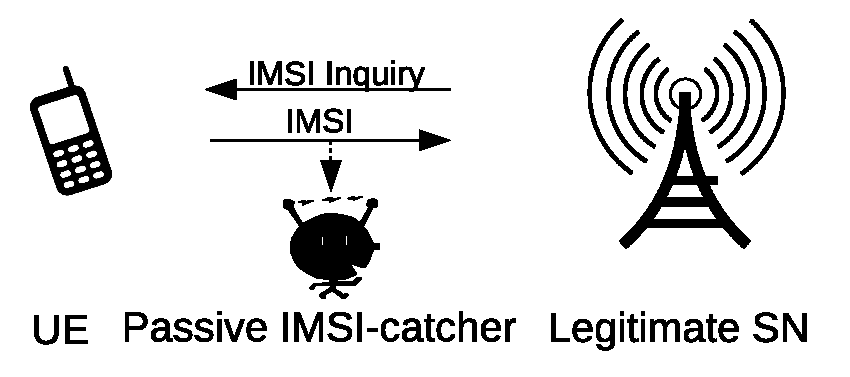
\includegraphics[width=\textwidth]{Passive_IMSI-Catcher.eps}
%    \caption{Legitimate SN}
%  \end{minipage}
%  \hfill
%  \begin{minipage}[b]{0.50\textwidth}
%    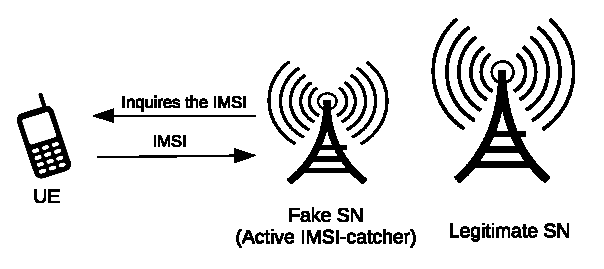
\includegraphics[width=\textwidth]{Active-IMSI-Cactcher.eps}
%    \caption{IMSI-catcher}
%  \end{minipage}
%  \caption{IMSI-catcher}
%  \label{fig:IMSI-catching}
%\end{figure}

\subsubsection{Our Contribution}
We propose a pseudonym based solution that builds on top of those in BVR, KM15 and KM17 schemes. The following contributions are made:
\begin{enumerate}
\item We show that a DoS attack can be mounted against an entire HN (when the BVR scheme is used) using the vulnerability identified in \cite{wisec17}. We calculate the expected success rate of the attack and argue that the attack can be fatal in practice.
\item We have identified weaknesses in KM17 scheme
\item We show how the synchronization of pseudonyms can be handled in a simple manner (also when there are DoS attacks), with three pseudonyms per user instead of six. In our solution, a UE can get a new pseudonym after using an old pseudonym only once in a successful AKA unlike the KM17 scheme. The KM17 scheme uses one pseudonym in two successful AKA runs.
\item Using probabilistic analysis, we show that a malicious SN can not mount any meaningful pseudonym desynchronization attack against our solution.
\item We discuss some practical concerns of using pseudonyms instead of IMSIs from billing and lawful interception point of view and suggest solutions.
\end{enumerate}




\section{Preliminaries}
From a hight level, a cellular network consists of $3$ elements. A UE, SN and HN. The SN and HN are the same network when the user is not roaming. An SN or HN consist of many entities. In this paper we will not discuss those fine details. However, we need to know some detail about a UE. A UE consists of two entities. A mobile equipment (ME) and a subscriber identity module (SIM). The SIM is known as universal subscriber module (USIM) in UMTS. SIM or USIM, they are smart cards which are portable across different MEs. In LTE, the USIM is an application in the universal integrated circuit card (UICC). In this paper, for the sake of simplicity we will refer all of them as SIM.


A user is identified by IMSI. IMSI is a string of $15$ decimal digits. An IMSI is a concatenation of mobile country code (MCC), mobile network code (MNC) and mobile subscription identification number (MSIN). MCC is a string of $3$ decimal digits. MNC is of $2$ to $3$ decimal digits and MSIN is of $9$ to $10$ decimal digits. Pseudonyms discussed in this paper are IMSI looking strings. In this paper we limit our discussion to only one HN. Consequently all the IMSIs or pseudonyms we discuss have the same MCC and MNC. When we talk about IMSI space or pseudonym space, we actually mean the MSIN space. We denote the size of this space by $\mathcal{M}$. The value of $\mathcal{M}$ can be either $10^9$ or $10^{10}$. We will also use $n$ to denote the total number of users subscribed with an HN.

In the cellular networks, the security is built on a pre-shared master key $\mathcal{K}$ between a user and its HN. The key $\mathcal{K}$ is stored in the SIM along with the IMSI. The HN maintains a map from IMSI to key $\mathcal{K}$ for all the users. The authentication mechanism used by an SN to authenticate a user is based on challenge and response. The the key $\mathcal{K}$ is only known by the HN, hence the HN delegates the SN by sending the challenge and expected response. We will soon describe the authentication mechanism in UMTS and LTE briefly. But before that, we mention the use of temporary mobile subscription identity (TMSI) and globally unique temporary UE identity (GUTI).

Once a user is authenticated by the SN, the user is given a temporary identity by the SN with confidentiality protection. The temporary identity is used by the SN and UE thereafter to identify the user so that anyone listening to the radio traffic can not identify the user. The temporary identity is known as TMSI in GSM and UMTS networks, and as GUTI in LTE network. The use of TMSI and GUTI can not defeat the IMSI catchers because the SN can still make an IMSI inquiry to a UE. Hence an IMSI catcher impersonating a legitimate SN can also make an IMSI inquiry. 

TMSI or GUTI is assigned to a UE by the SN. They are assigned with confidentiality protection after the authentication is successful and necessary security context has been set up. However, pseudonyms are assigned by the HN and no security context is set up between a UE and an HN after authentication. Hence, the idea is to assign the pseudonym to a user during the authentication. This requires to make certain changes in the authentication protocol. In UMTS and LTE, the authentication protocols are called UMTS AKA and LTE AKA respectively. LTE AKA has a very little difference compared with UMTS AKA. Before we discuss the pseudonym based solutions, we present UMTS AKA  and LTE AKA briefly.

\subsection{UMTS/LTE AKA}
We discuss UMTS and LTE AKA only very briefly so that we can make a smooth transition to the discussion of pseudonym based solution. Details of UMTS AKA can be found in clause 6.3 of 3GPP TS 33.102 \cite{TS33102} and LTE AKA can be found in clause 6 of 3GPP TS 33.401 \cite{TS33401}. 

The UE identifies itself using the IMSI to the SN while sending an attach request or responding to an IMSI inquiry. Upon receiving the IMSI, an SN sends an authentication vector (AV) request to the HN for the IMSI. The HN finds the pre-shared key $\mathcal{K}$, randomly generate a challenge ($RAND$) and compute the expected response ($XRES$), two keys $CK$ and $IK$ as function of $\mathcal{K}$ and $RAND$. The HN also computes a string called $AUTN$ for the purpose of some cryptographic protections of the authentication protocol. HN forwards $RAND,AUTN,XRES, CK,IK$ to the SN. SN forwards the $RAND,AUTN$ to the UE. The UE verifies the $AUTN$, computes $SRES,CK,IK$ using the $RAND$ and key $\mathcal{K}$ and forwards $SRES$ to the SN. If $SRES$ and $XRES$ are the same strings, then the authentication is successful. The keys $CK$ and $IK$ are used for confidentiality and integrity protection thereafter. See Figure \ref{fig:UMTS_LTE_AKA}.

In LTE, upon receiving the AV request, the HN also computes another key $K_{ASME}$. And unlike UMTS, the HN forwards $RAND,AUTN,XRES,K_{ASME}$ to the SN. The UE verifies the $AUTN$, computes $SRES,CK,IK, K_{ASME}$ using the $RAND$ and key $\mathcal{K}$ and forwards $SRES$ to the SN. If $SRES$ and $XRES$ are the same strings, then the authentication is successful. The key $K_{ASME}$ is used to generate further keys for confidentiality and integrity protection. See Figure \ref{fig:UMTS_LTE_AKA}.

\begin{figure}[]
  \centering
    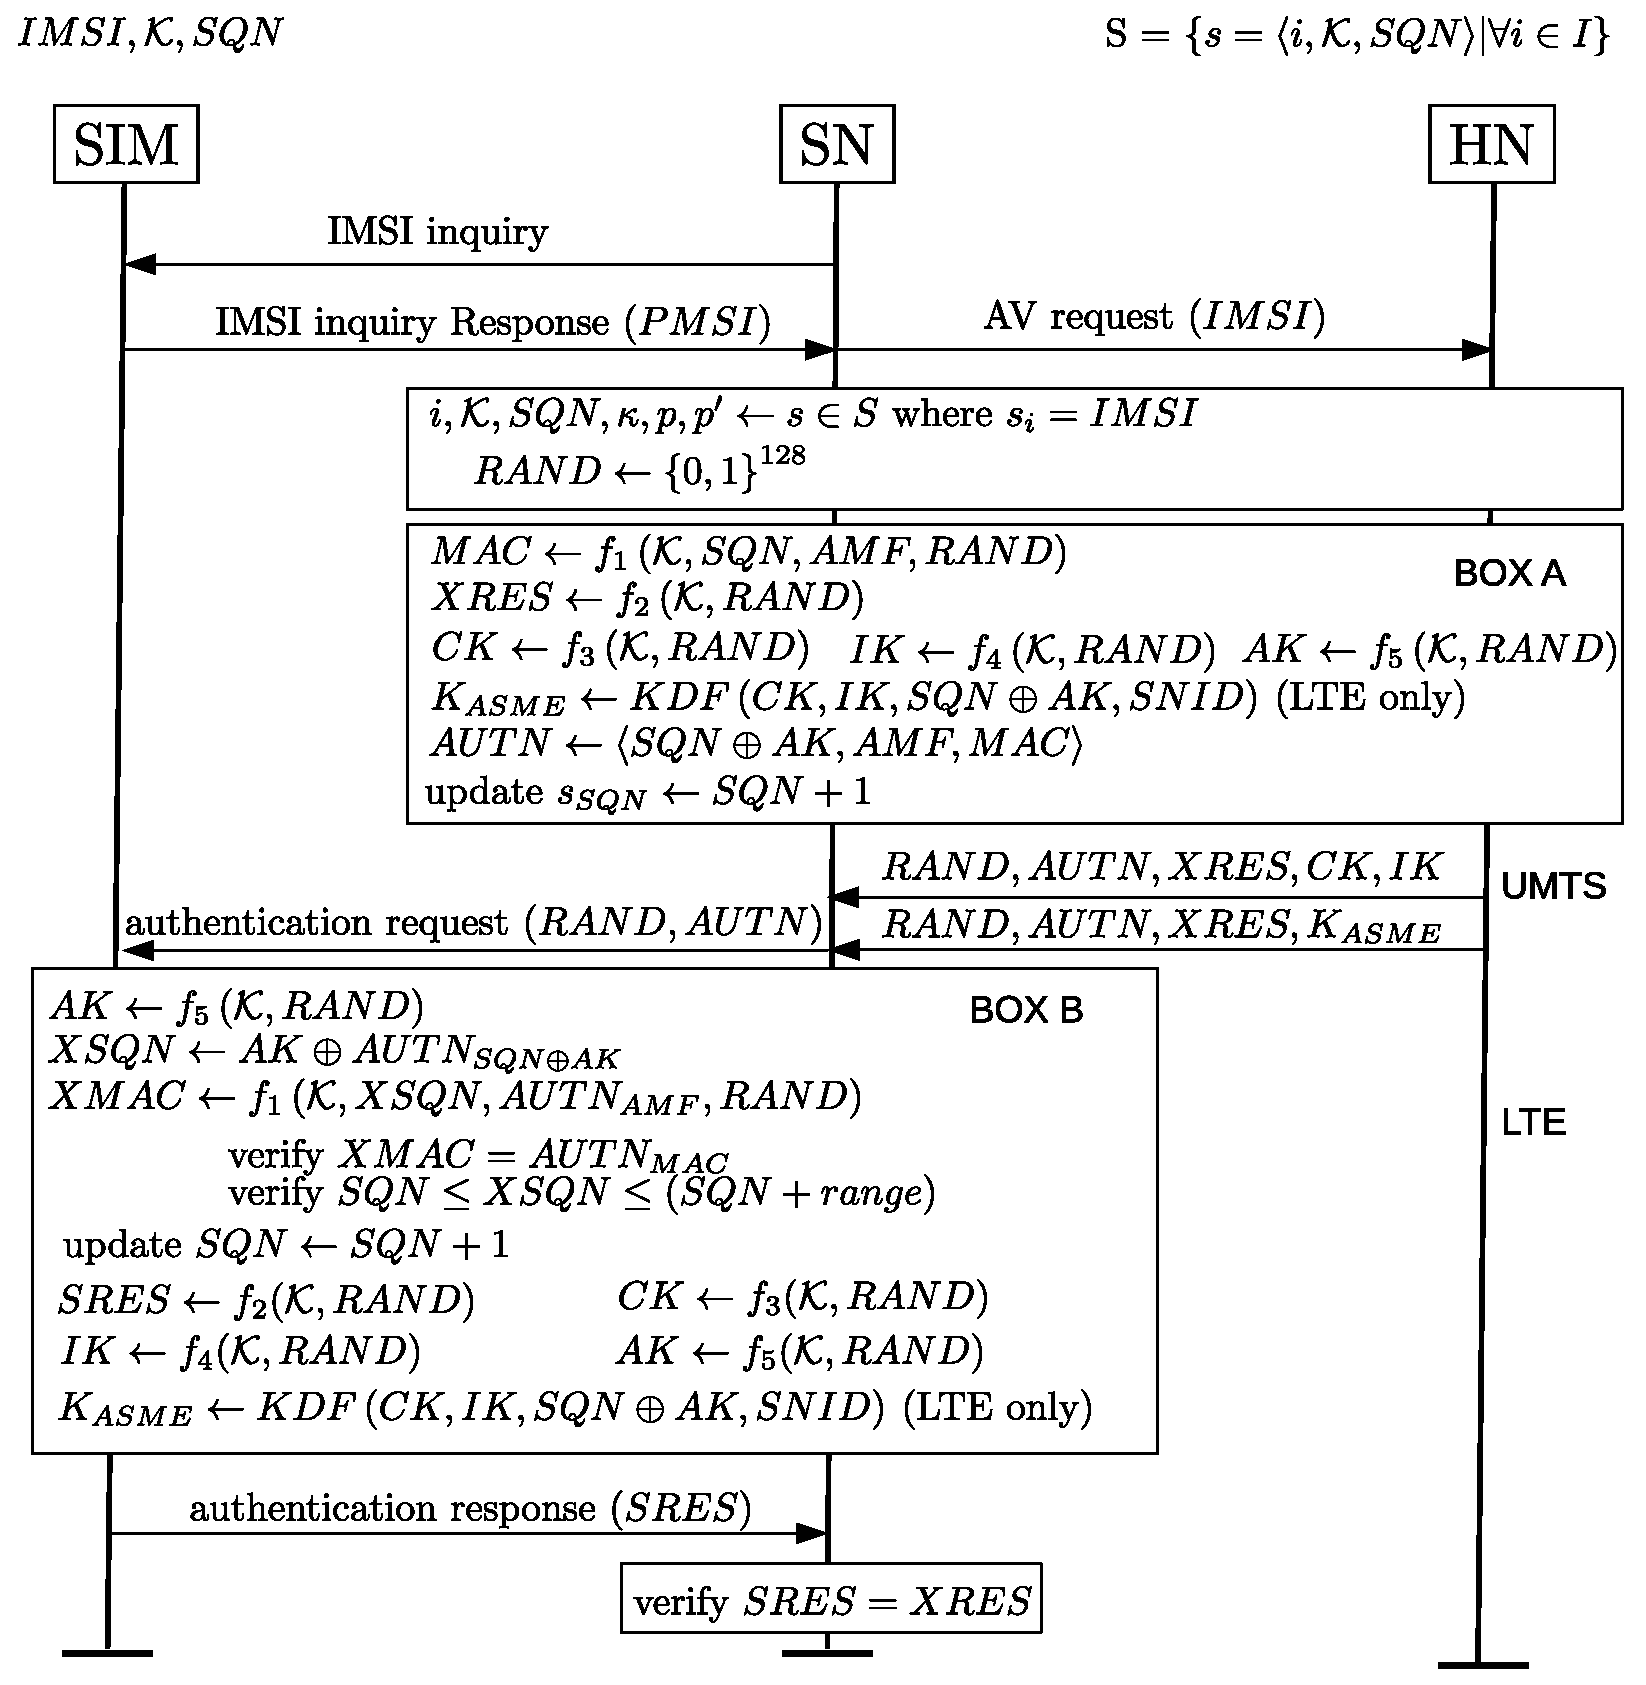
\includegraphics[width=.9\textwidth]{UMTS_LTE_AKA.eps}
  \caption{UMTS/LTE AKA}
  \label{fig:UMTS_LTE_AKA}
\end{figure}

\subsection{Location Update} It is specified in 3GPP TS 23.012 (Section 3.6.1.1) \cite{TS23012}, that, when a UE registers with a visitor location register (VLR), an entity in the SN, the  VLR provides its address to the home location register (HLR), an entity in the HN. When a UE uses an IMSI/pseudonym for the first time, it is considered as a registration in the SN and consequently the HN is informed with the address of the SN for the IMSI/pseudonym. We will refer to this location update message sent for IMSI/pseudonym $x$ as $\text{LU}_{x}$ in this paper. We will use these LU messages in our solution.


\section{Related Work}
The BVR and KM schemes describe how the use of HN recongnized pseudonym can be introduced in the legacy networks. Following the BVR and KM15 schemes in 2015, there have been few other proposals \cite{Ginzboorg_Niemi_2016,Norrman_Naslund_Dubrova_2016,yemen2017} published in 2016 and 2017. All these proposals use essentially the same idea of using frequently changing pseudonyms recongnized by the HN. The vulnerability identified in \cite{wisec17} is present in all these solutions. So, for simplicity and limitation of space, we choose and explain only one of these schemes briefly and present our attack and solution in the context of the chosen scheme. We choose the BVR scheme.

\subsection{BVR Scheme}
They pseudonym used in this scheme is called pseudo mobile subscriber identifier (PMSI). Besides the shared secret $\mathcal{K}$, every user shares another secret key $\kappa$ with the HN. The SIM inside the UE stores two pseudonyms at any point of time, $\left(PMSI,P_{new}\right)$. The SIM uses $P_{new}$ the next time the UE receives an IMSI inquiry and keep using $P_{new}$ until it receives a new pseudonym. The HN also stores two pseudonyms $\left(p,p'\right)$ for every subscriber at ay point of time. In an ideal situation, $PMSI = p$ and $P_{new} = p'$. 

The HN sends the next pseudonym encrypted by the key $\kappa$ as a part of the random challenge $RAND$ used in AKA. Upon the successful and positive completion of the AKA between the SN and the UE, the next pseudonym can be decrypted by the SIM. The BVR scheme builds on top of the UMTS/LTE AKA. Figure \ref{fig:bvr_solution} shows the required changes. Comparing Figure \ref{fig:UMTS_LTE_AKA} and \ref{fig:bvr_solution} shows that no changes are made in the messages that are transmitted, but only in the end points, i.e., the SIM and the HN. Since both of the HN and the SIM are maintained by same entity, the scheme is transparent to the legacy SNs.


\begin{figure}[]
  \centering
    \includegraphics[width=.9\textwidth]{BVR.eps}
  \caption{The BVR Scheme}
  \label{fig:bvr_solution}	
\end{figure}


\subsubsection{Vulnerability in BVR Scheme}
Note that, whenever an AV request arrives for $p'$, the HN forgets $p$. Forgetting an old pseudonym is important so that it can be reused. But forgetting before being confirmed that $p'$ has been received by the UE is a vulnerability as pointed in \cite{wisec17}. If a fake UE (FUE) identifies itself using a random pseudonym and if by chance, the random pseudonym is associated with a legitimate UE, the HN forgets an old pseudonym for the legitimate UE. The network also computes a new pseudonym which the legitimate UE has no knowledge of. If the network remembers  $k$ number of pseudonyms before forgetting any, the FUE needs to make the attack $k$ times so that the network forgets all the pseudonyms that the legitimate user possesses. So, in the case of BVR scheme, the FUE has to send two pseudonyms. This is a fatal damage to the identity of the UE, because all the successive authentications of the UE will fail. In Section \ref{sec:attack} we will show how this vulnerability can be exploited into a fatal DoS attack.


\subsection{KM17 Scheme} \label{sec:km17scheme}
In KM17, the authors have used the LU messages sent by an SN to an HN after registration of a new IMSI as the confirmation that the UE has received $p'$. The scheme uses three pseudonyms in the HN instead of two. It also uses three recovery identities (RID), that we will discuss in the following section.


\subsubsection{Weaknesses in KM17 Scheme}
Careful investigation in KM17 scheme shows that a pseudonym has to be used at least two times before the UE can get a new pseudonym from the HN. The scheme maintains three pseudonyms $p_{past},p_{current}$ and $p_{future}$ at the HN end. The HN always embeds encrypted $p_{future}$ (generates a new one if $p_{future}$ is null) in the RAND. The HN forgets $p_{past}$ only when $\text{LU}_{p_{future}}$ arrives at HN. $\text{LU}_{p_{future}}$ would arrive only if $p_{future}$ was used by the UE already at least once. After receiving $\text{LU}_{p_{future}}$, the HN updates $p_{past} \leftarrow p_{current}$, $p_{current} \leftarrow p_{future}$ and $p_{future} \leftarrow null$. Now, the UE has to use $p_{current}$ to get a new pseudonym from the HN. Notice that the $p_{current}$ after the location update is same as the $p_{future}$ before the location update arrived. Consequently, our claim follows.

The authors argue that the scheme is not immune to malicious SN who tries to attack by sending fake LU messages. As a reactive measure, the authors propose a recovery process that enables a UE and the HN to get back in a synchronized state of pseudonyms. The scheme uses temporary recovery identity (RID). The HN sends the RID as a part of the RAND in a similar way a pseudonym is sent. When a UE gets convinced that the pseudonym synchronization has been lost, the UE sends the RID piggybacked in the reject message AUTS. Based on the RID, the process can recover to a synchronized pseudonym state. Detail of the process can be found in \cite{wisec17}. However, an IMSI catcher can convince a UE that the synchronization has been lost and learn the RID of the UE. Now the IMSI catcher can track the user using this RID instead of IMSI. This argument shows that the pseudonyms used in this scheme are as good as frequent the RIDs are changed. 

However, one might argue that the RIDs can be changed as frequent as the pseudonyms are changed. Note that, forgetting an old RID is also triggered by the same location update message that triggers forgetting an old pseudonym. Consequently, synchronization of RIDs become as vulnerable as synchronization of pseudonyms, when a malicious SN sends fake location update message.

\section{Attack On BVR Scheme} \label{sec:attack}
The attack is mounted by an FUE. The attack has two phases.

\subsubsection{Phase 1} \label{sec:attac_fue_phase1}  An FUE sends an attach request using a random pseudonym $q_1$ to a legitimate SN. The legitimate SN sends an AV request for $q_1$ to the HN. If by chance, $q_1 = p'$, the HN forgets $p$ and sets $p \leftarrow p'$. The HN also generates an unused pseudonym $p''$ and sets $p' \leftarrow p^{''}$. As a result, in the HN, the current  pseudonym-state for the subscriber $s$ is $\left(p = P_{new},p' \notin \left\lbrace PMSI,P_{new} \right\rbrace \right)$. %See Figure \ref{fig:dos_attack}.

\subsubsection{Phase 2} \label{sec:attac_fue_phase2} The FUE sends another attach request using a random pseudonym $q_2$ to a legitimate SN. The legitimate SN sends a AV request for $q_2$ to the HN. If again by chance, $q_2 = p'$, then the HN again forgets $p$, sets $p \leftarrow p'$. HN also generates an unused pseudonym $p'''$ and sets $p' \leftarrow p'''$. Consequently, the current pseudonym-state of subscriber $s$ is $\left\lbrace PMSI,P_{new} \right\rbrace \cap \left\lbrace p,p' \right\rbrace = \emptyset$. %See Figure \ref{fig:dos_attack}

%\begin{figure}[]
%  \centering
%    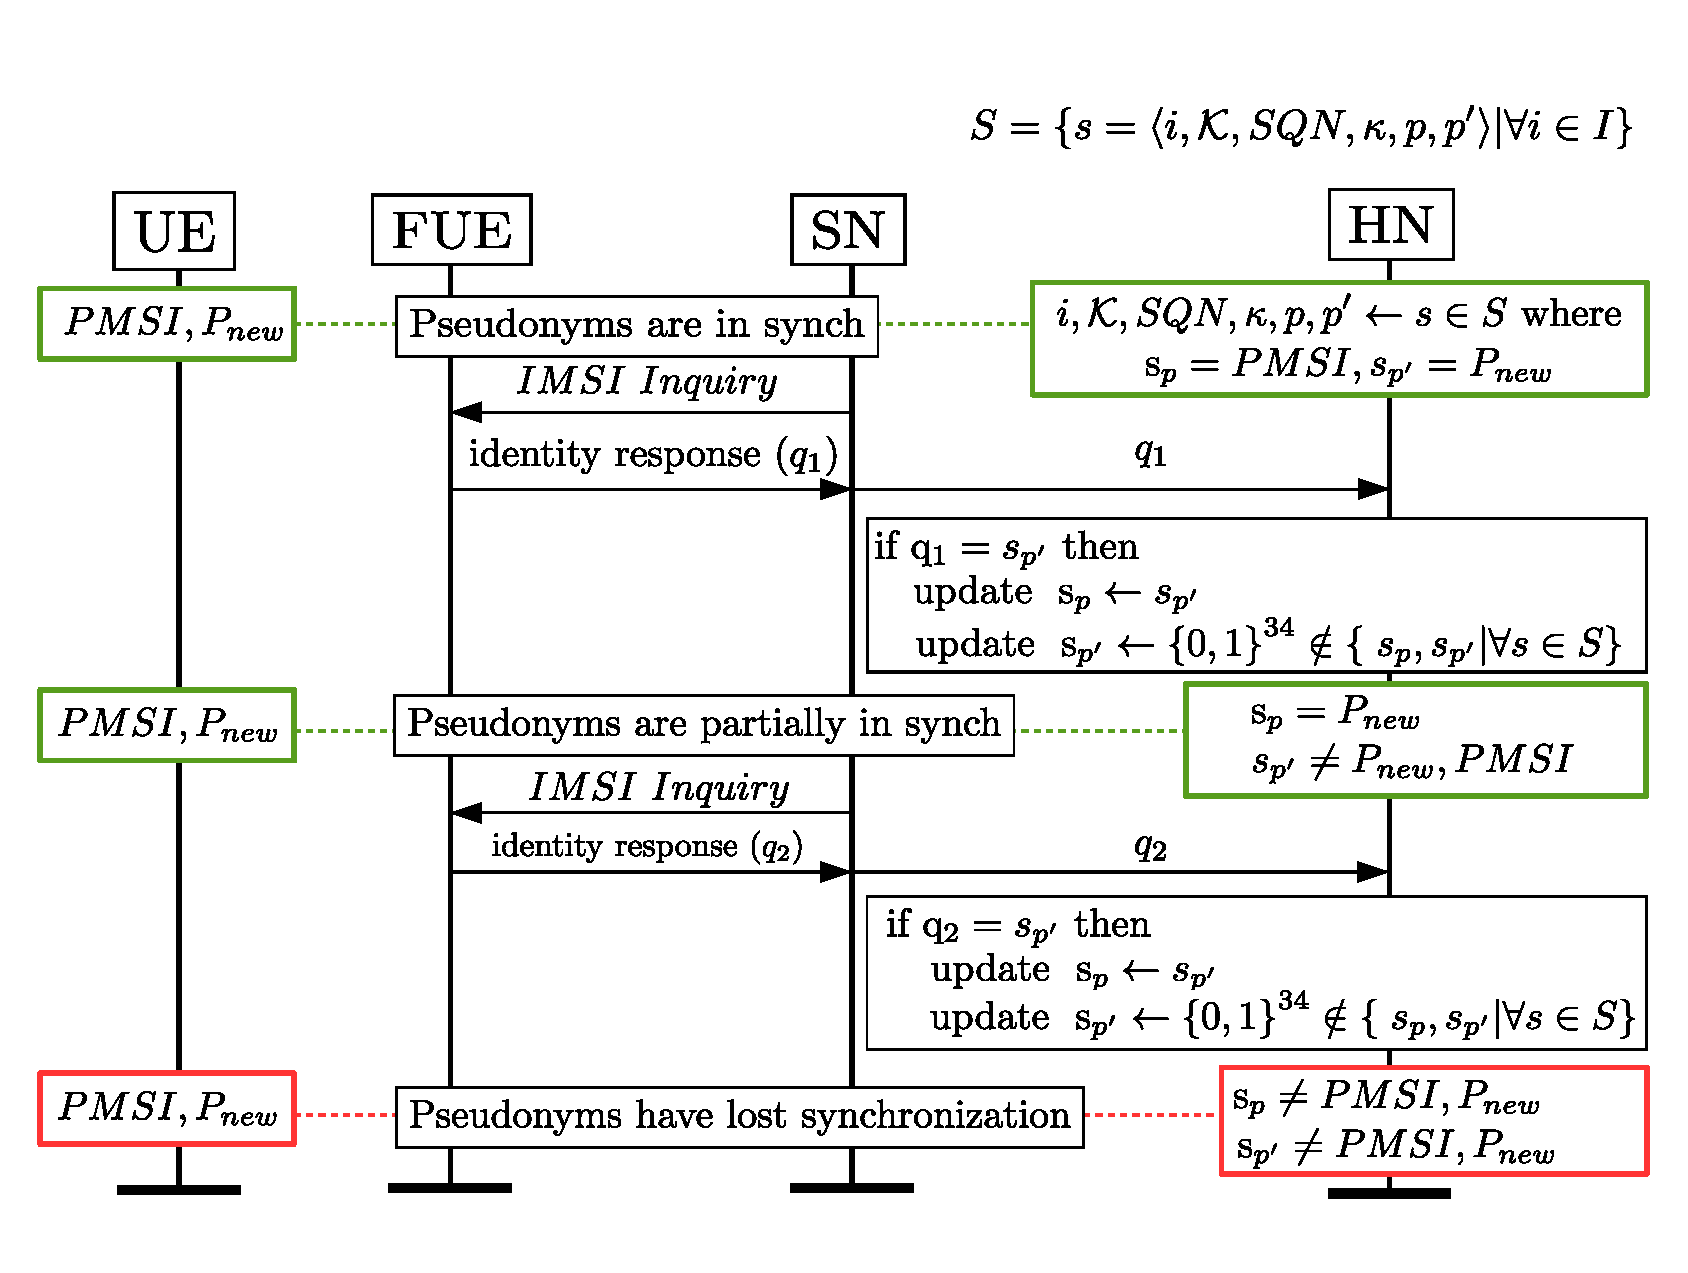
\includegraphics[width=.9\textwidth]{DDoS.eps}
%  \caption{A DoS Attack against the BVR scheme}
%  \label{fig:dos_attack}	
%\end{figure}

The next time the user would need to authenticate itself to a network, the authentication will fail and hence be denied any service. In this attack, it is assumed that the UE has not obtained a new pseudonym via a legitimate SN while the attack was mounted.

\subsection{The DDoS Attack Against the BVR Scheme} \label{sec:ddos_attack}
The DDoS attack is mounted by a botnet of mobile devices. The mobile bots send many attach requests using different pseudonyms to legitimate SNs. The legitimate SNs in turn sends AV request for those pseudonyms to the HN. Let us assume, the total number of pseudonyms sent to the HN is a large integer $m$. In this case, a user $s$ will be affected by the attack if there exists two integers $0 < x < y \leq m$ such that $q_{x} = s_{p'}$ and $q_{y} = s_{p'}$. 

We have considered two different ways to mount this attack. In one way, the pseudonyms used in the attach requests are chosen randomly with replacement, which means the attack might sent one pseudonym more than once to the HN. In the other way, the pseudonyms are chosen without replacement, which means the attack send one pseudonym only once.

\subsubsection{With Replacement}
In this case, after sending $m$ number of pseudonyms to the HN, the expected portion of affected users $E[u_a]$ is
\begin{eqnarray}
E\big[ u_a \big] &=& \left(1- \left(1 - \frac{1}{\mathcal{M}}\right)^m - m\left(\frac{1}{\mathcal{M}}\right)\left(1 - \frac{1}{\mathcal{M}}\right)^{\left(m-1 \right)} \right) \label{eqn:avg_with_replacement}
\end{eqnarray} 

See Appendix \ref{appendix: A} for the derivation. We have run a simulation of this attack and found that above model is fairly accurate. See Figure \ref{fig:simulation_and_modeling}.


\begin{figure}[]
  \centering
  \begin{minipage}[b]{0.49\textwidth}
    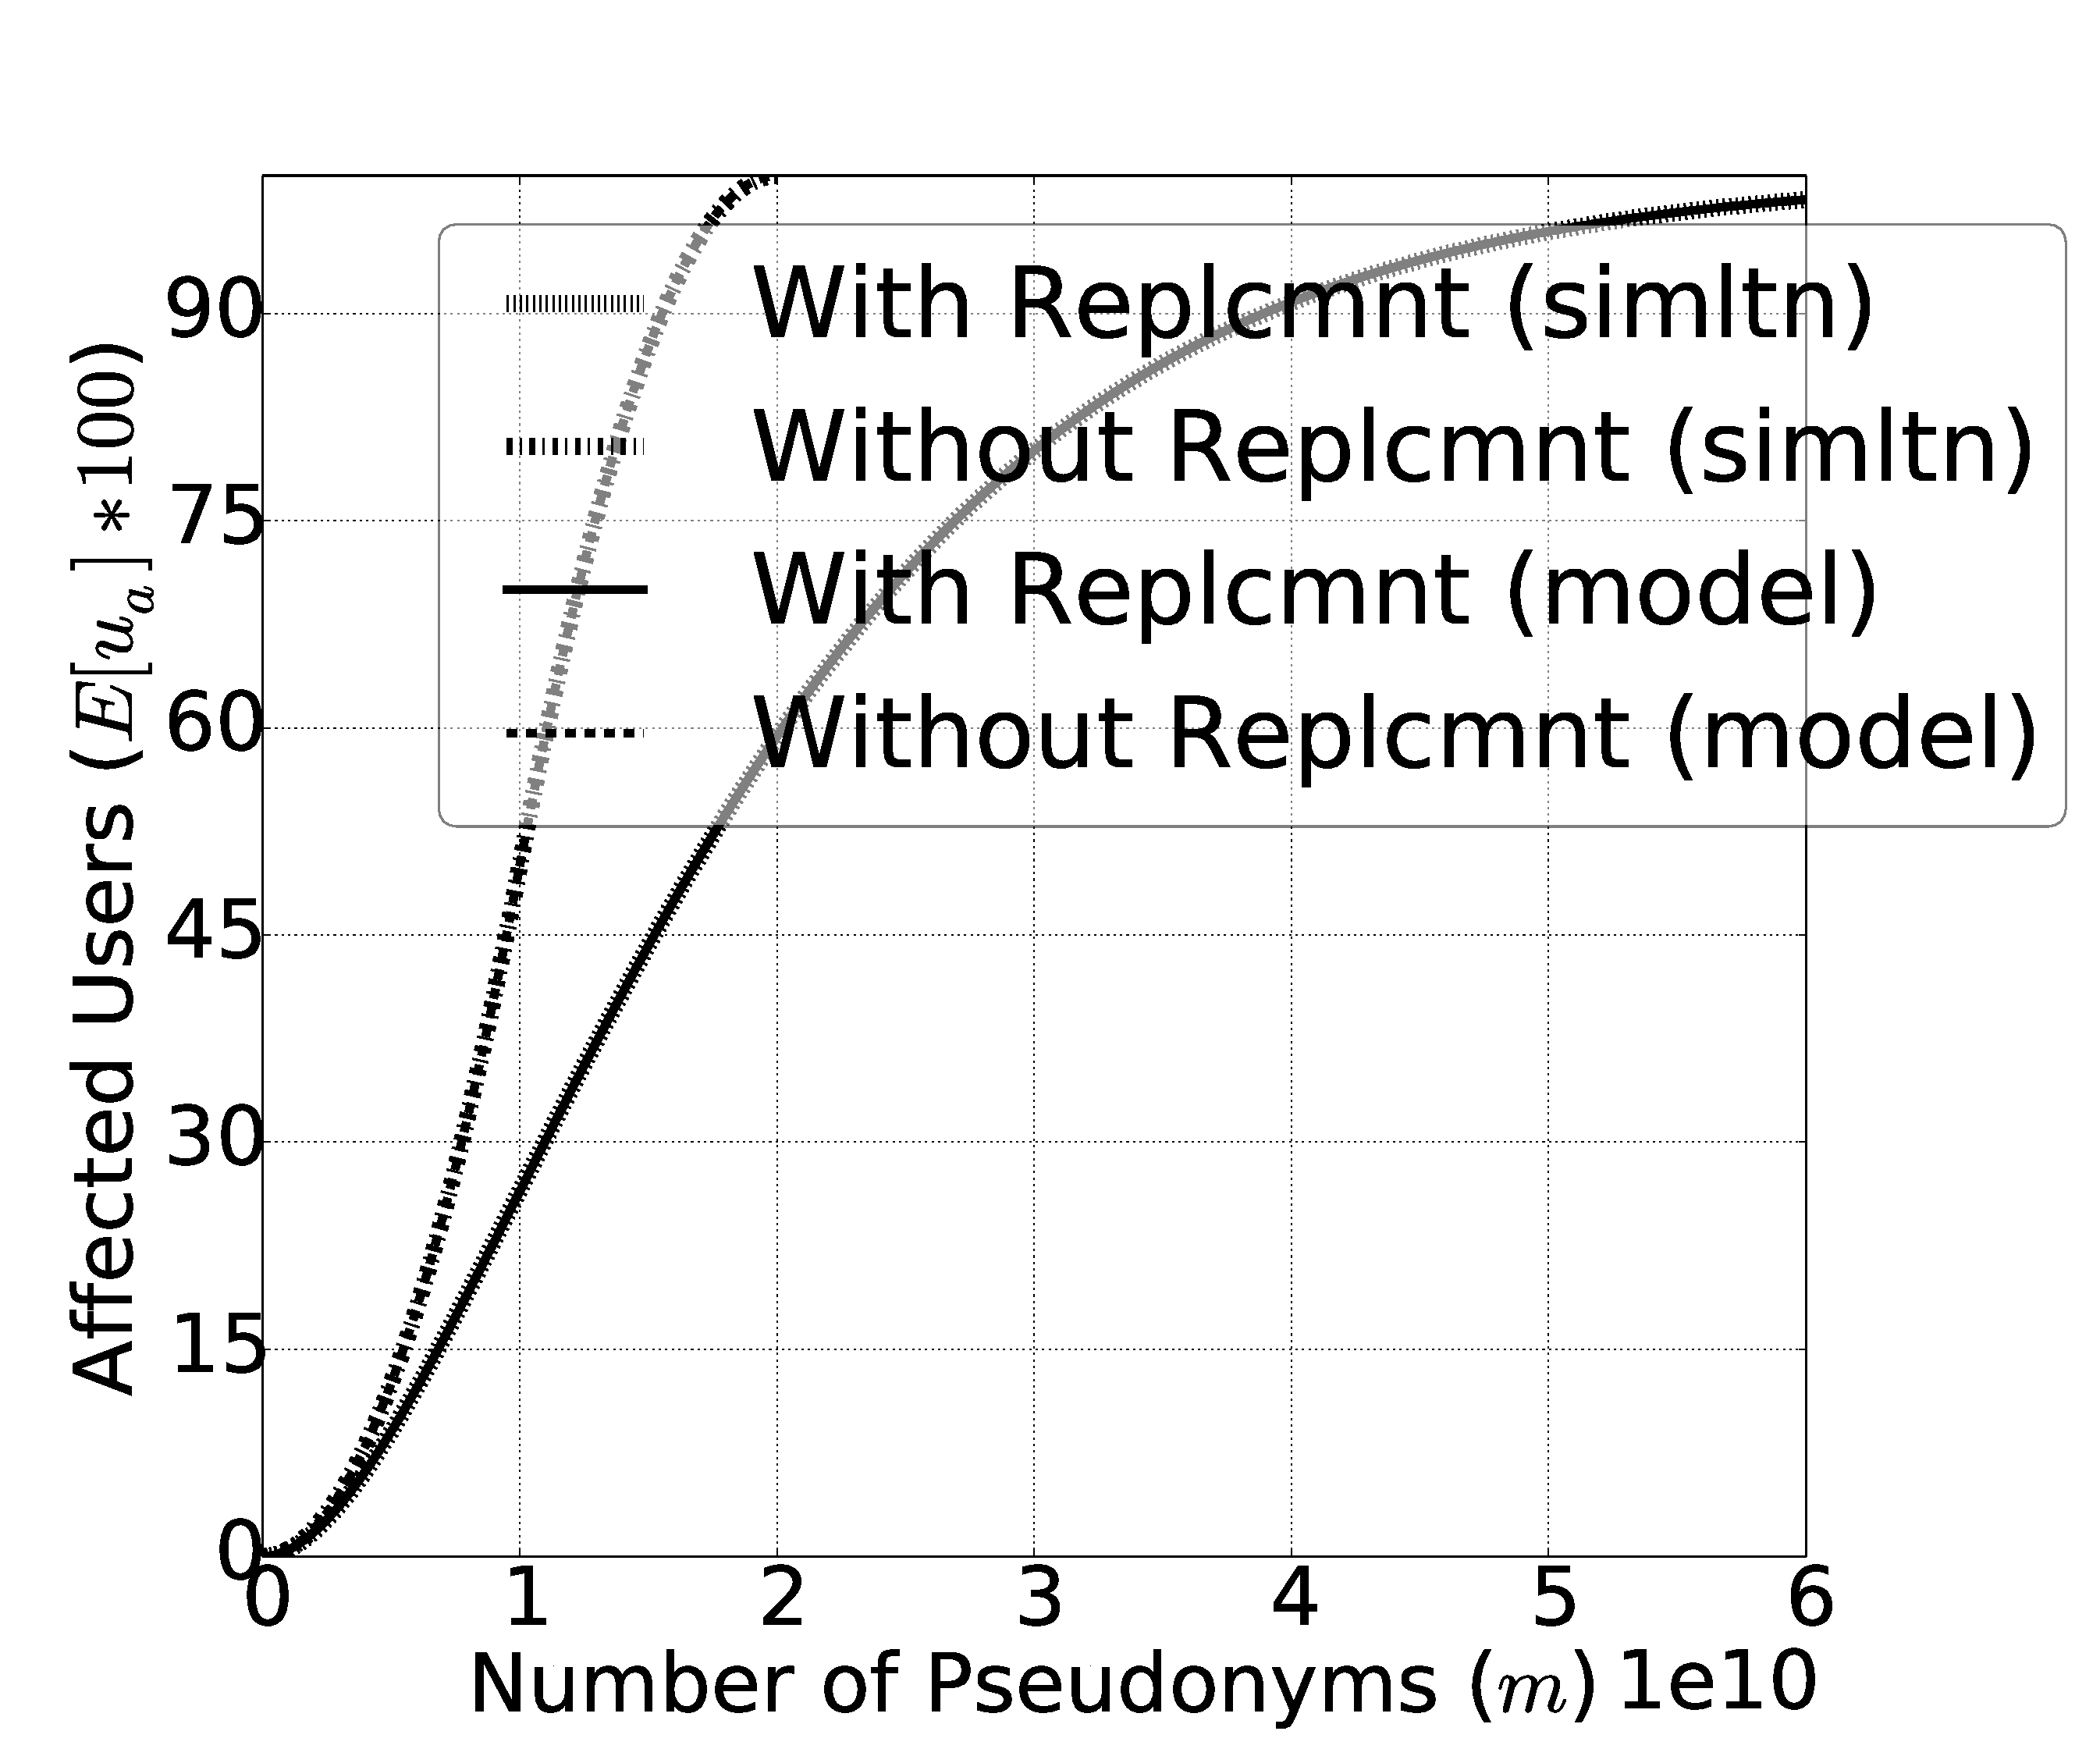
\includegraphics[width=\textwidth]{sim_and_mod.pdf}
   \caption{DDoS Attack. $ \mathcal{M} = 10^{10}, n = 10^{7}$. The model fits so well that it is difficult to distinguish the empirical lines from the model.}
\label{fig:simulation_and_modeling}
  \end{minipage}
  \hfill
  \begin{minipage}[b]{0.49\textwidth}
    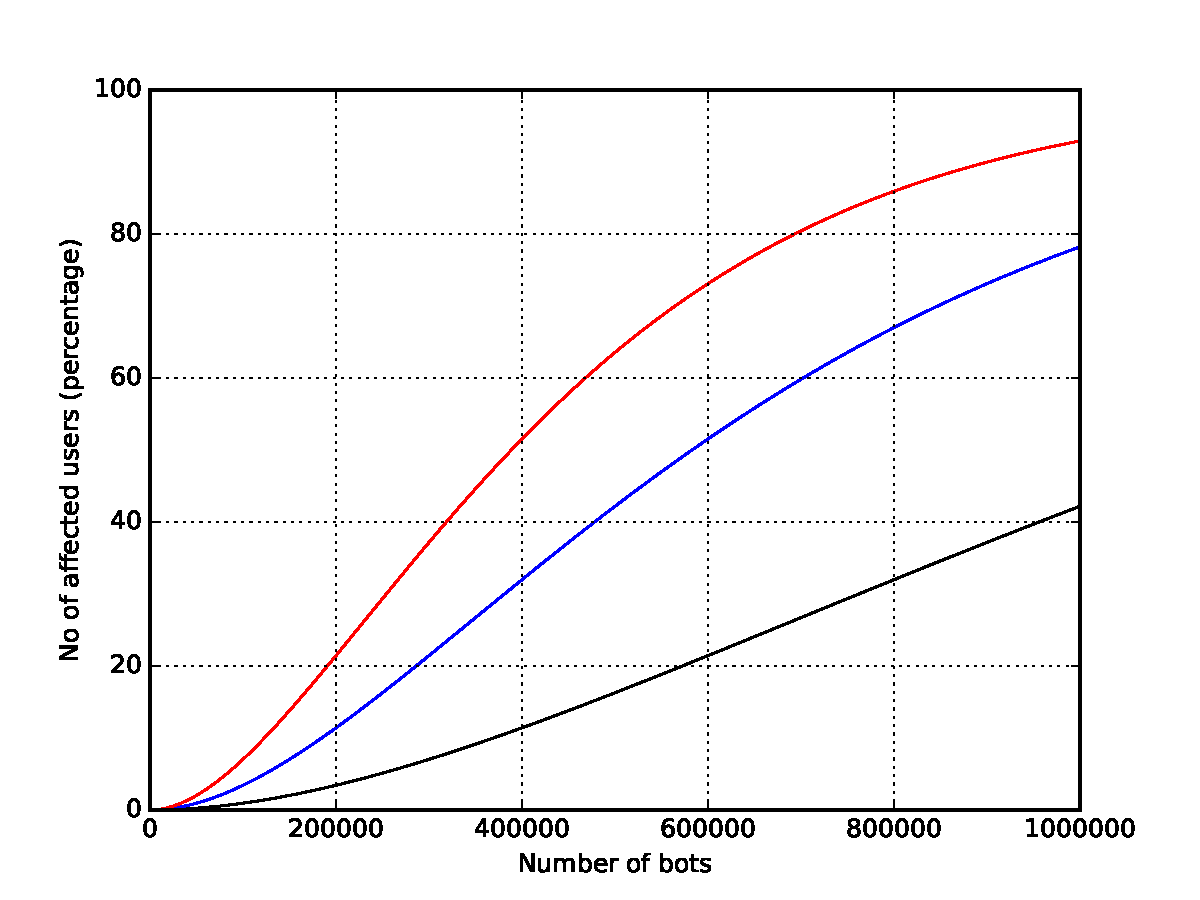
\includegraphics[width=\textwidth]{botplot.pdf}
    \caption{DDoS Attack (with replacement), $\texttt{botnet}_{\texttt{size}} = 10^6$. Different lines represent the success rate as $\texttt{bot}_{\texttt{load}}$ varies.}
  \label{fig:botplot}
  \end{minipage}
\end{figure}

\subsubsection{Without Replacement}
In this case the attacker runs two rounds of the attack. In the first round the attacker sends all the pseudonyms in the IMSI space without replacement, means each pseudonym is sent exactly once. Once the first round is completed, the attacker runs the attack for one more round. However, after sending $m$ number of pseudonyms to the HN, the expected portion of affected users $E[u_a]$ is
\begin{eqnarray}
E\big[ u_a \big] = \begin{cases} \frac{1}{\mathcal{M}}\frac{m^2}{2\cdot \mathcal{M}} & \mbox{if } 0 < m \leq \mathcal{M} \\ 
\frac{1}{\mathcal{M}}(2m - \mathcal{M} - \frac{m^2}{2\mathcal{M}}) & \mbox{if } \mathcal{M} < m \leq 2\mathcal{M} \end{cases}
\label{eqn:without_replacement}
\end{eqnarray} 

See Appendix \ref{appendix: A} for the derivation. We have run a simulation of this attack and found that above model is fairly accurate. See Figure \ref{fig:simulation_and_modeling}. Note that, this is an estimation where the without-replacement attack is not a distributed attack. Rather the attack is mounted by only a single FUE. In the case of distributed and without replacement attack, the expected perecentage of affected users will be less than what is shown in the plot. However, we believe that, the distributed and without replacement attack will have higher number of affected users than that of distributed with replacement attack. %However, it can be a strategic decision of the attacker to choose the value of $\texttt{bot}_{\texttt{load}}$.


\subsection{How Fatal The DDoS Attack Can be In Practice} \label{sec:how_fatal_ddos}
The intensity of the attack in practice will depend on two parameters. The first one is the size of the botnet, we name as $\texttt{botnet}_{\texttt{size}}$. The second one is the number of pseudonyms a bot sends per unit time in the attach requests, we name as $\texttt{bot}_{\texttt{load}}$. According to a thesis conducted in Lund University in 2016 \cite{thesislund}, the EPS AKA has the latency of $550$ milliseconds even when the MME is far away (10,000 km) from the HN. So, the peak value of $\texttt{bot}_{\texttt{load}}$ can safely be considered as $1$ pseudonyms/second, i.e., 3600 pseudonyms/hour.

Mobile botnets are on the rise \cite{botnet_ccs09_symbian,botnet_usenix11,botnet_australia_2016}. Many mobile botnets have already been observed, e.g., Geinimi \cite{botnet_geinimi10}, Zeus \cite{botnet_zeus11}, AnserverBot \cite{botnet_anserverbot}, DreamDroid \cite{botnet_dreamdroid11}. A detailed survey of the state of mobile botnets can be found in \cite{botnet_threat15}. In 2011, it was estimated that Dreamdroid was installed on 120,000 mobile devices \cite{botnet_dreamdroid11}. In 2014, a mobile botnet of 650,000 mobile phones made an attack to a server \cite{chinese_spam}. It would not be surprising if we see a mobile botnet consisting tens of millions of mobile bots in near futrue. However, for the discussion of this paper, we conservatively set the variable $\texttt{botnet}_{\texttt{size}} = 1$ million ($10^6$). See Figure \ref{fig:botplot}, it shows how efficient a botnet of size $10^6$ can be for varied values of $\texttt{bot}_{\texttt{load}}$.

\begin{figure}[]
  \centering
    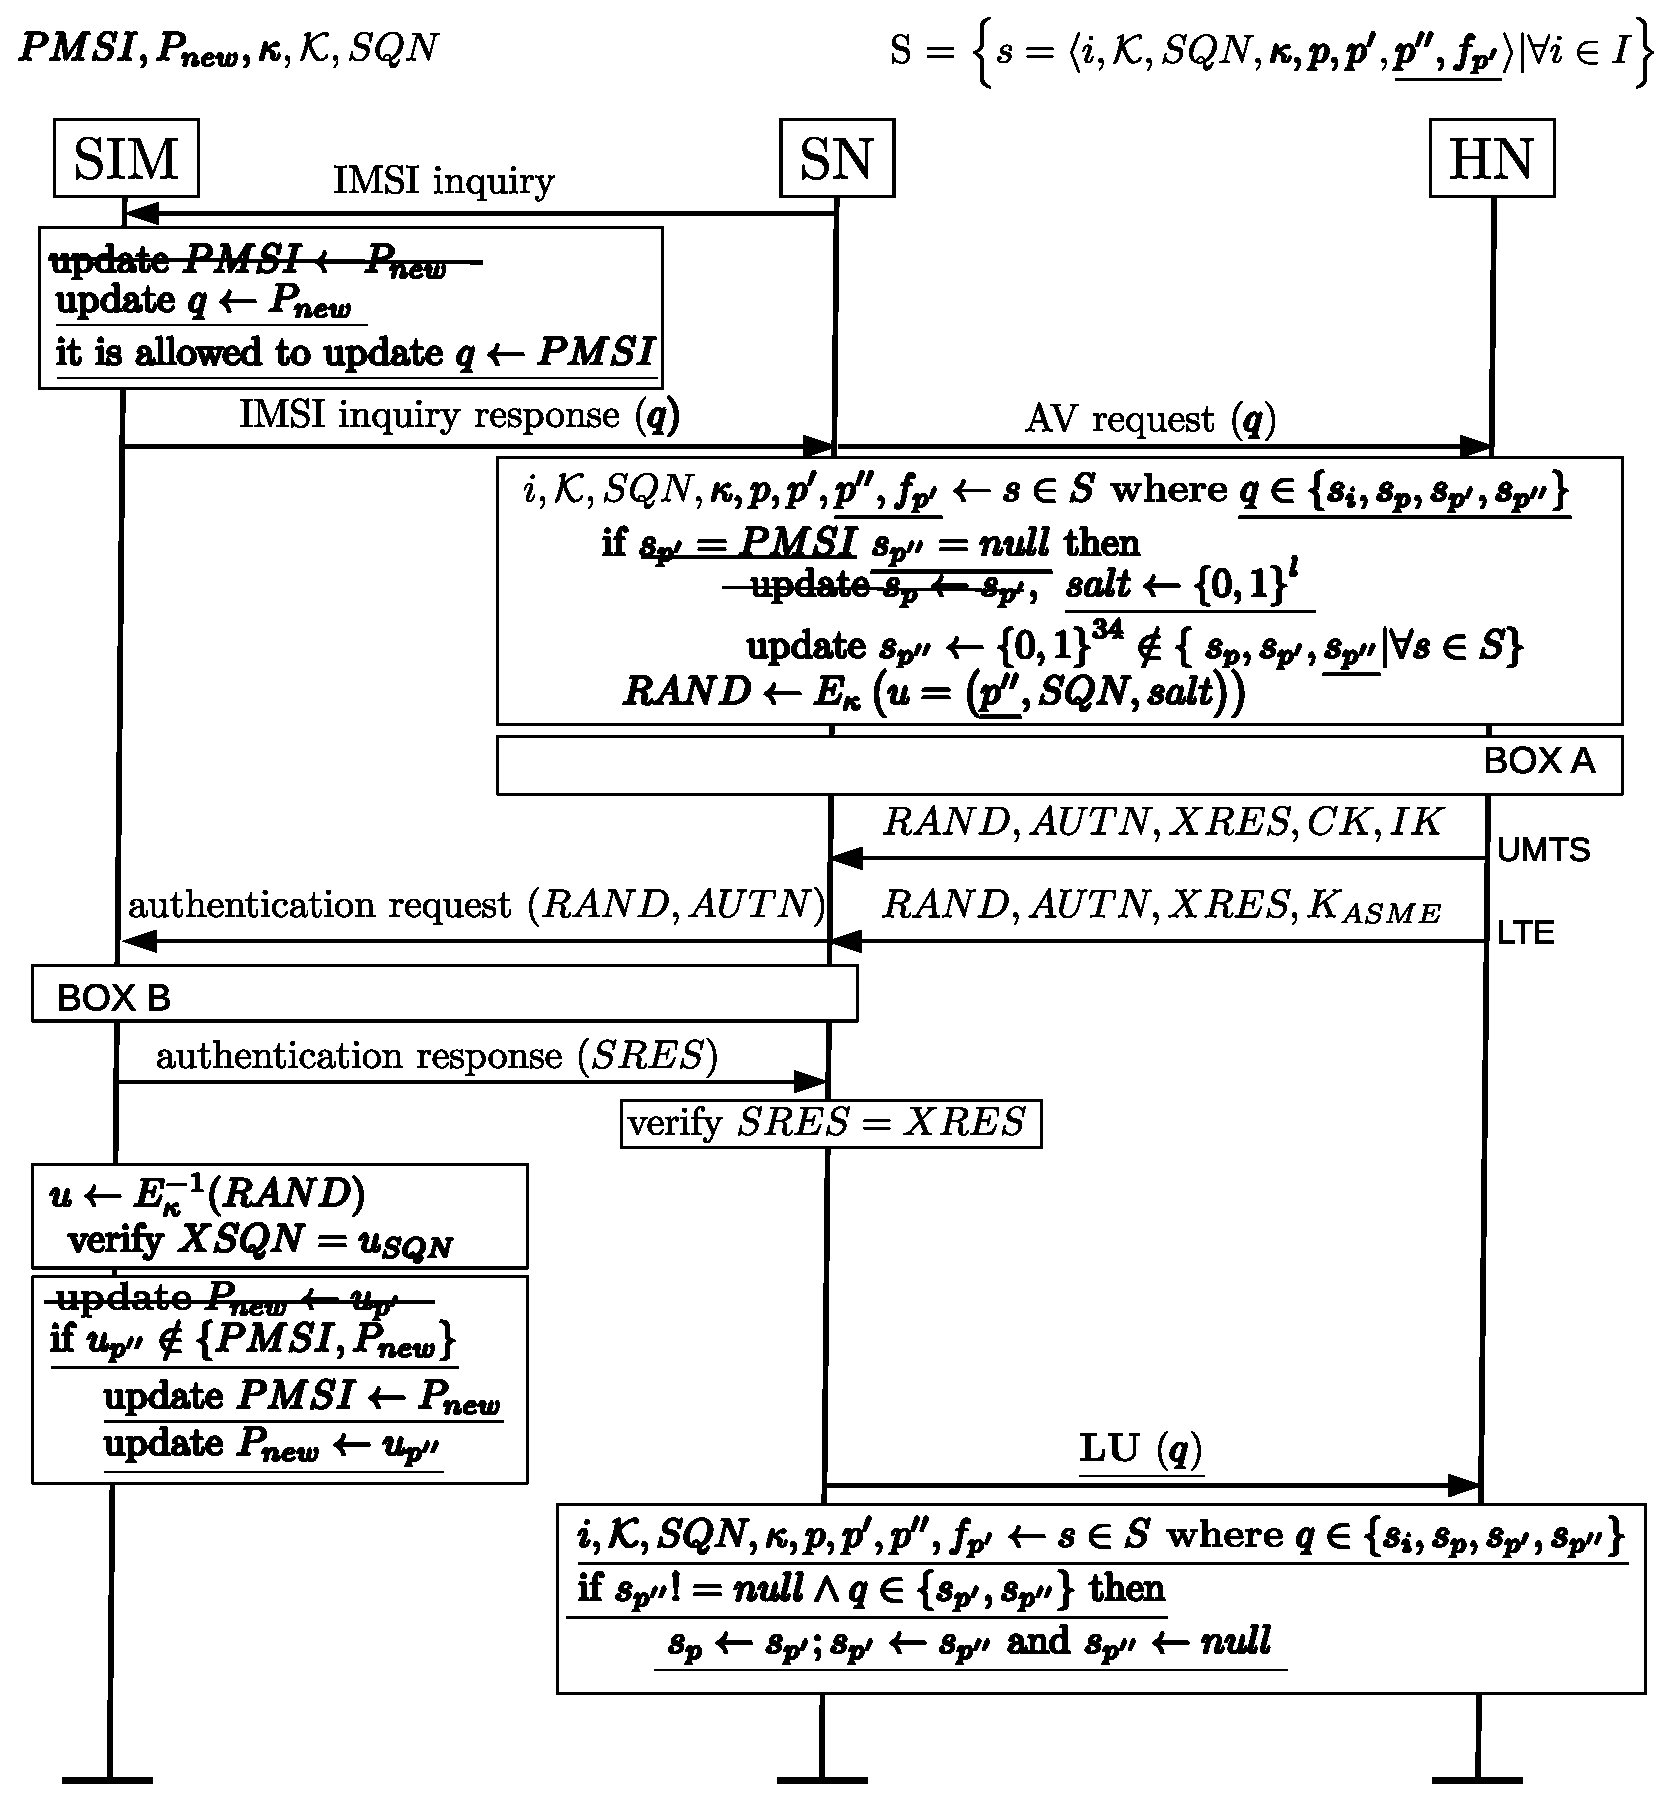
\includegraphics[width=\textwidth]{solution.eps}
  \caption{Solution}
  \label{fig:solution}	
\end{figure}

\section{Our Solution}
\begin{enumerate}
 \item discuss the solution where the UE will be asked if it want to share the IMSI.
\end{enumerate}
As in the KM17 scheme, our solution also uses the location update message sent by an SN to the HN after the successful and positive completion of an AKA. In the legacy networks, the location update message is sent for an IMSI. As the pseudonyms and IMSIs are not distinguishable by an SN, the location update messages will be sent by an SN for the pseudonyms too. Let us assume that for a subscriber $s \in S$ an AV request has arrived using the pseudonym $p$ and the HN has responded with an AV by embedding $p'$ in the RAND. When a location update for pseudonym $p$ arrives, the HN considers it as the guarantee that pseudonym $p'$ has been delivered to the UE of user $s$.

In the HN, for a user $s \in S$, our solution stores the IMSI $i$ and three pseudonyms $p,p',p''$. In the UE of the user $s$, two pseudonyms $PSMI,P_{new}$ are stored. In an ideal situation $PMSI = p, P_{new} = p'$. We build our solution on top of the BVR scheme. Figure \ref{fig:solution} presents our solution. The bold texts present the changes over UMTS. The bold stricken out texts present the parts that we have discarded from the BVR scheme. The bold and underlined texts present the parts that we have added. 


\subsubsection{At HN side}
Whenever an AV request is received for a subscriber $s$, using any of its identity, i.e., $i,p,p'$ or $p''$, the HN responds with an AV that contains a pseudonym $p''$ in the RAND. If $p''$ is $null$ then an unused pseudonym is chosen and set as $p''$. When $p''$ is not null and a location update message arrives using any of the identities $p',p''$, the HN forgets $p$ by setting $p \leftarrow p', p' \leftarrow p''$ and $p'' \leftarrow null$. 


\subsubsection{At UE side}
If $MAC$ and $SEQN$ verification is successful then the UE verifies if $u_{SEQN}$ is the same as the $XSEQN$. If this verifications is also successful and $P_{new} \neq p''$, then the UE sends the SRES to the SN, and sets $PMSI \leftarrow P_{new}$ and $P_{new} \leftarrow u_{p''}$.


\section{Analysis of Our Solution}

\textcolor{red}{explain the state diagram a little more, explain what happens if the location update is lost}

Complexity arises in our solution when the location update message is delayed, lost, or sent multiple times. Also in practice, the location update message for pseudonyms $p,p',p''$ might arrive in different order because of the inherent characteristics of IP networks. A malicious or buggy SN might send a location update message even when the corresponding AKA was failed or maybe not even run.
To understand, how our solution behaves in these different unusual but possible situations, we study the different categories of states of the HN based on the relevant variables.  

We categorize all the possible states of HN in two categories. The first category is the one where $p''$ is not null and the second category is the one where $p''$ is null. Based on these two categories, we draw a state diagram as presented in Figure \ref{fig:HN_UE_diagrams}. On the other hand, the UE has only one state. It always have two pseudonyms $PMSI, P_{new}$. However, $PMSI$ and $P_{new}$ may have have different values. There are four options these values can be chosen from: $p,p',p''$ and $ \notin \left\lbrace p,p',p''\right\rbrace$. 

Based on successful AKA in between the UE and the SN, the values of $PMSI, P_{new}$ may change in the UE. On the other hand the values of $p,p',p''$ may change due to the arrival of an AV request or a location update message at HN. The action taken by an HN upon receving an AV requst or location update message depends on the value of $p''$ (null or not null). Based on the different values $PMSI,P_{new},p''$ can obtain, our solution can have $32$ different states. Many of these states are never reachable. Figure \ref{fig:solution_diagram} shows the state diagram of our solution with $9$ reachable states out of the total $32$. 



\begin{figure}
\centering
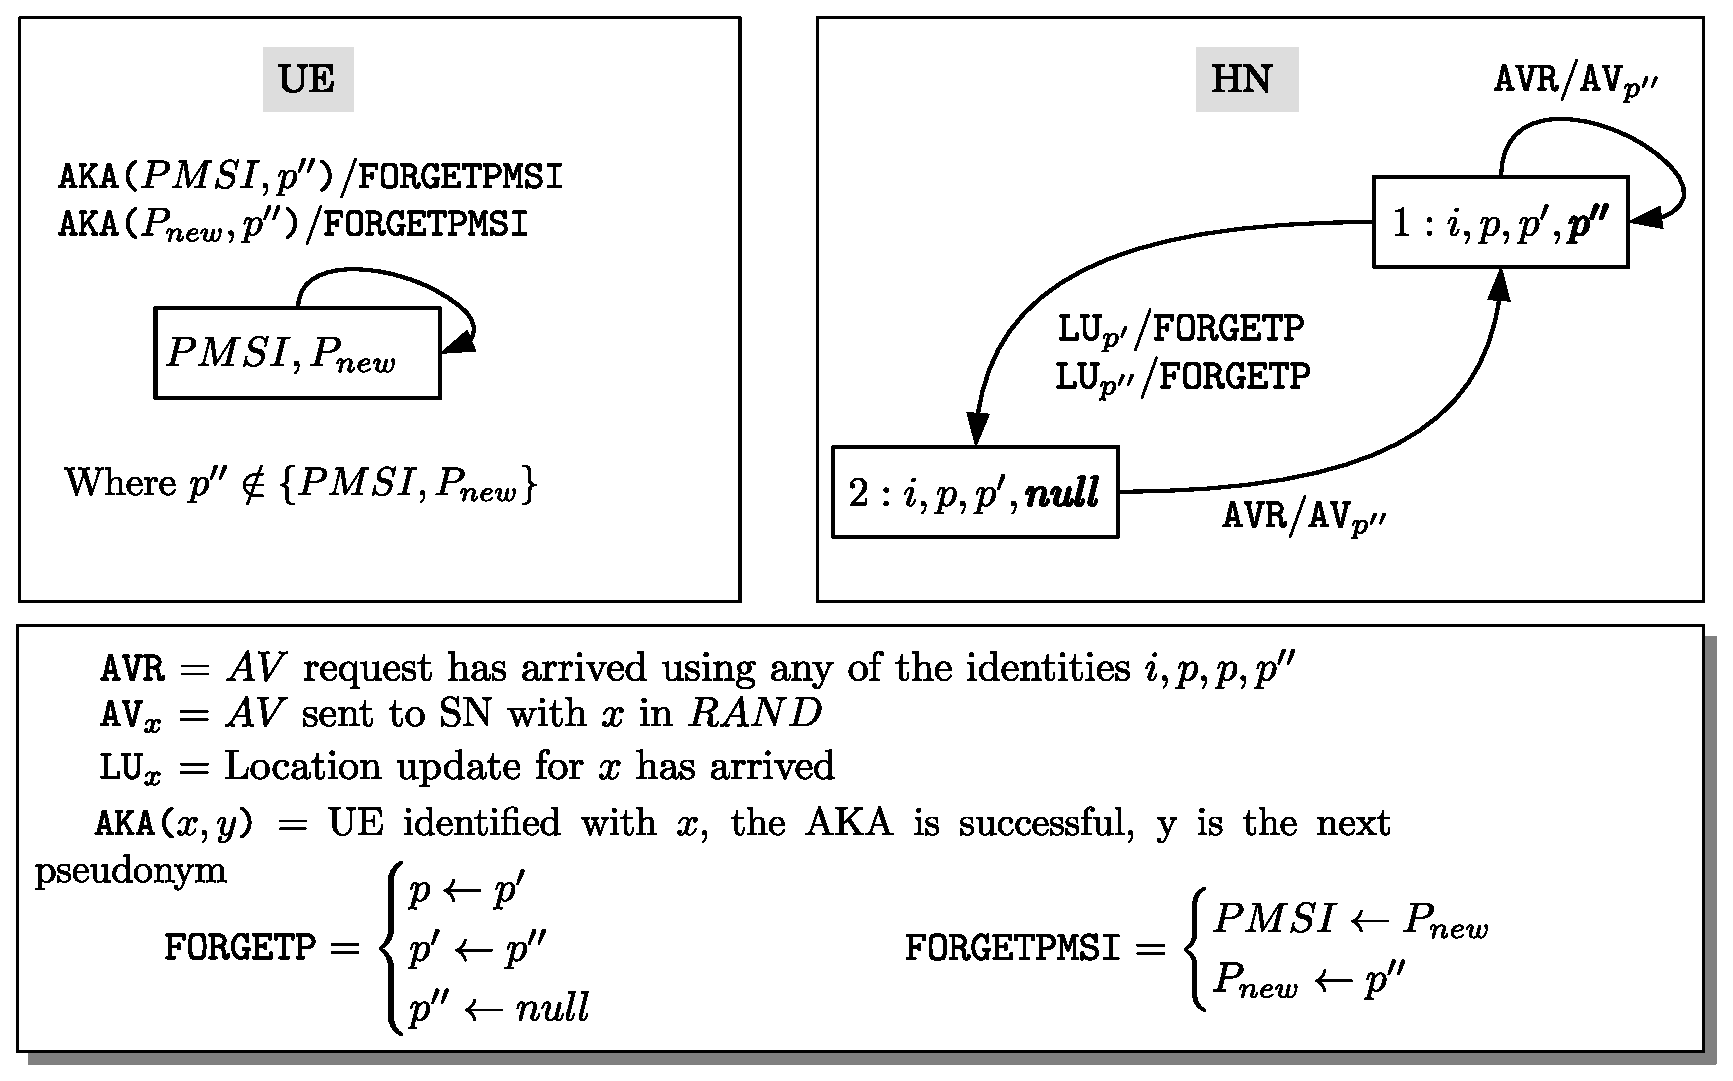
\includegraphics[width=.9\textwidth]{HN_UE_diagrams.eps}
\caption{State diagrams of UE and HN}
\label{fig:HN_UE_diagrams}
\end{figure}



\begin{figure}[!tbp]
  \centering
    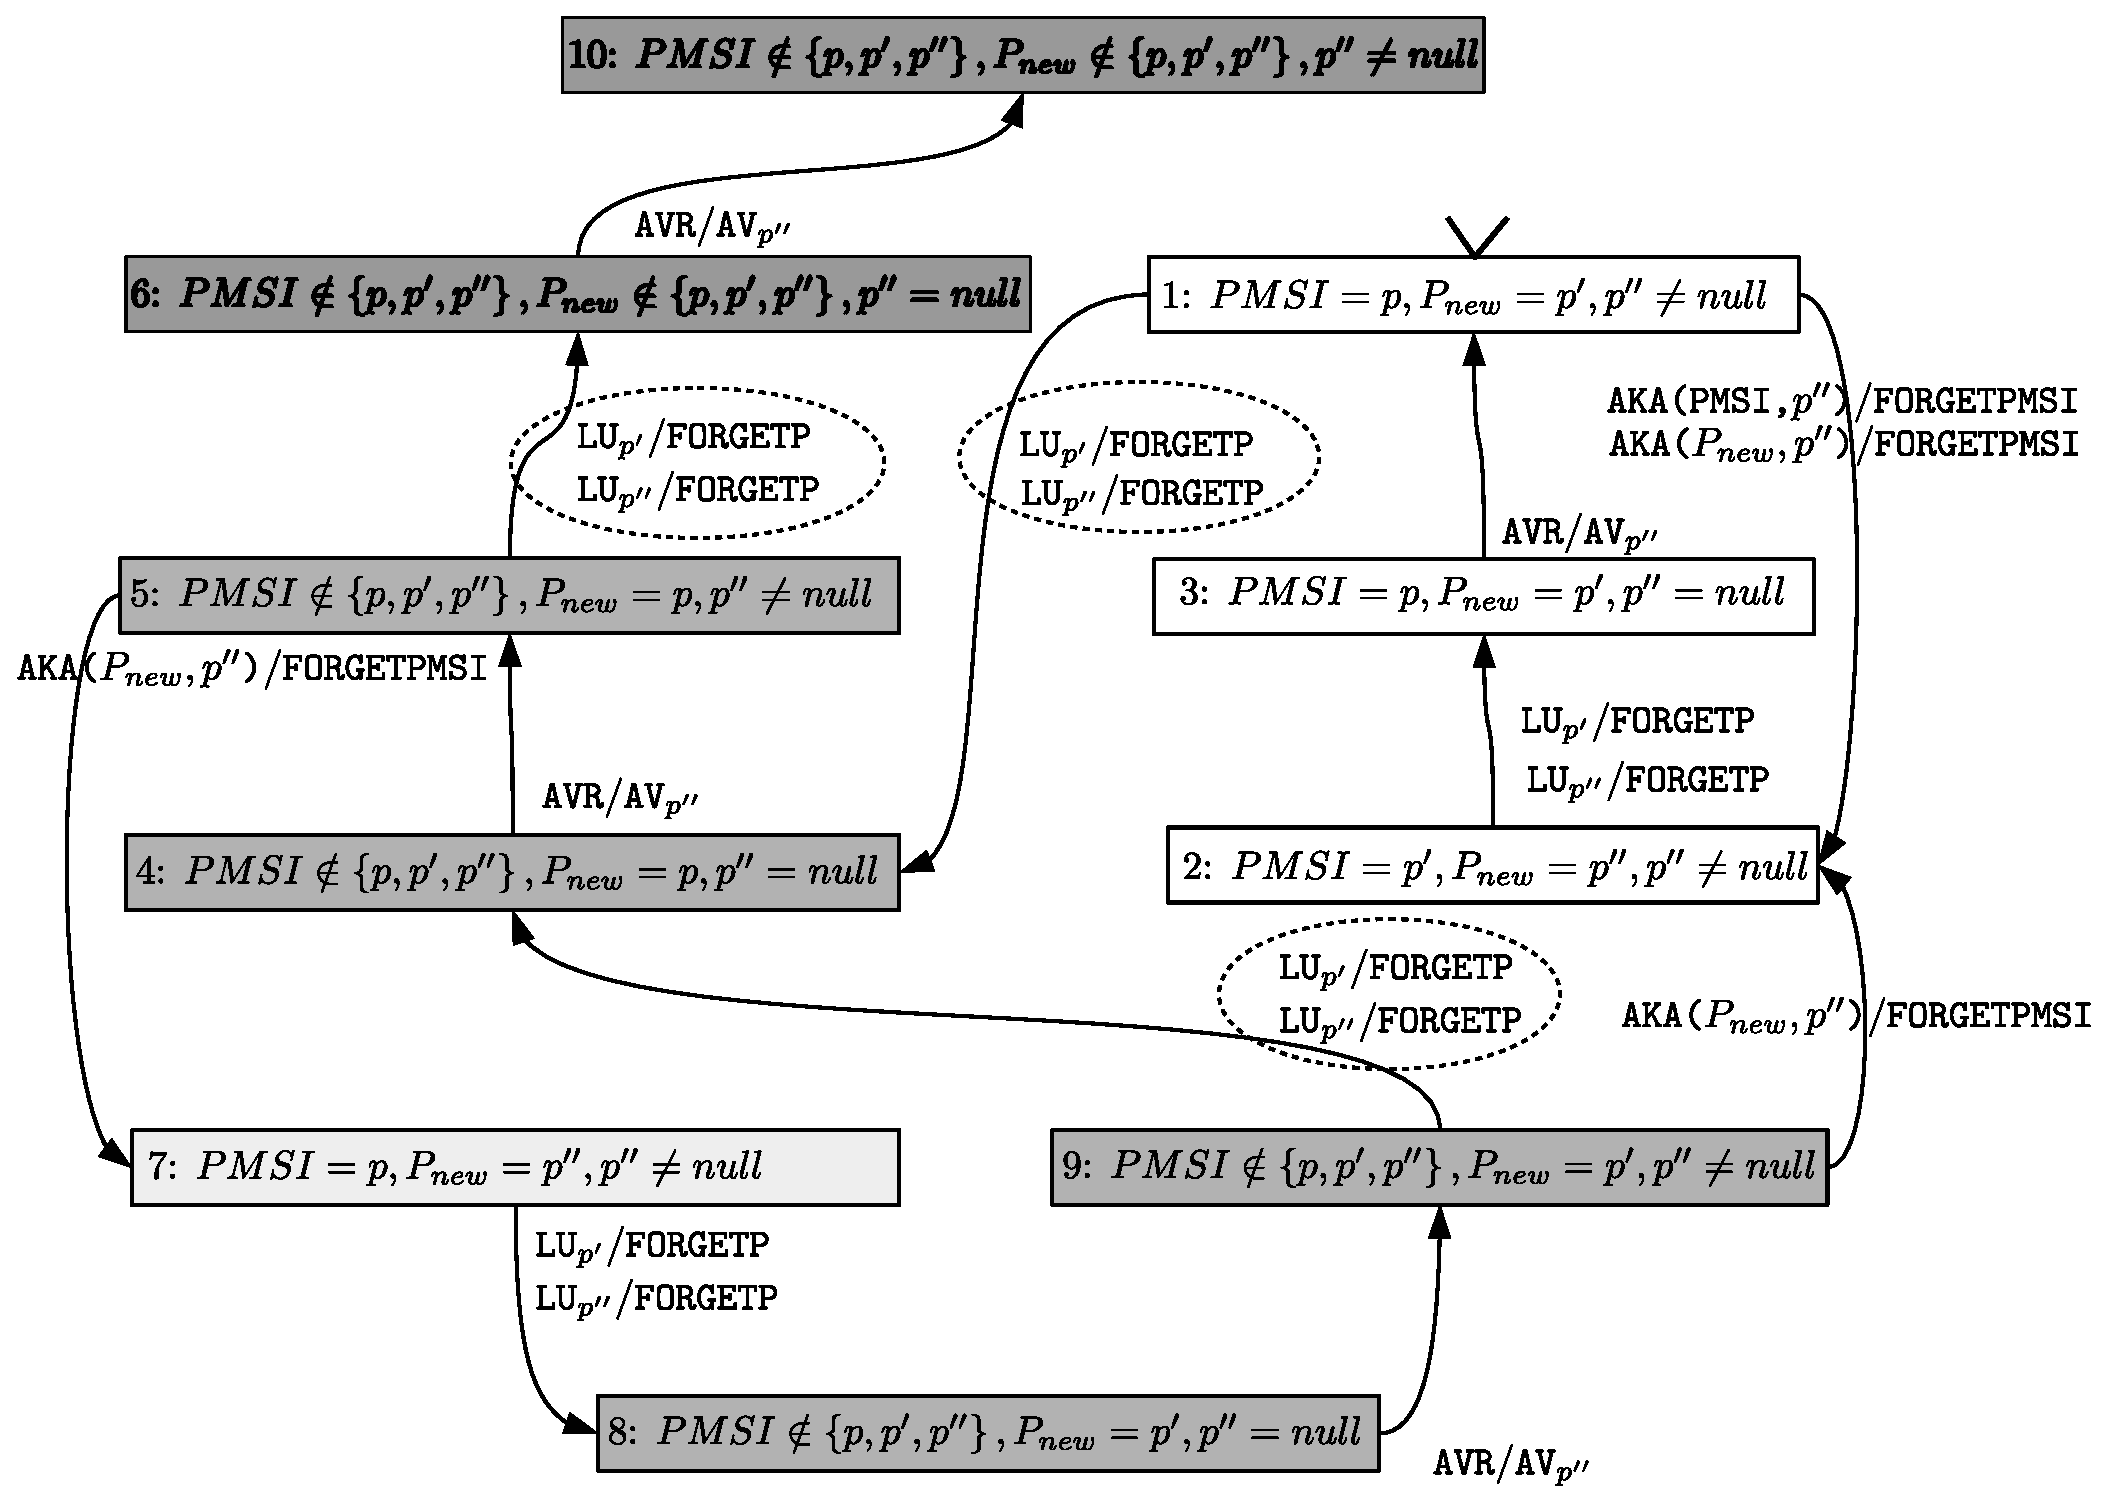
\includegraphics[width=.95\textwidth]{solution_diagram.eps}
 \caption{State diagram of our solution for a user $s \in S$. Neither the UE nor the HN has the knowledge in which state the the solution is. All a UE knows are two pseudonyms $PMSI,P_{new}$ and the HN knows three pseudonyms $p,p',p''$. Notations in Figure \ref{fig:HN_UE_diagrams} are also applicable here. The dotted circled LUs are sent by malicious or buggy SNs.}
  \label{fig:solution_diagram}
\end{figure}



\subsection{Protection Against IMSI Catcher} The pseudonyms are delivered to the UE encrypted by the pre-shared symmetric key $\kappa$. So, nobody except the UE can know the next pseudonym the UE will use. Hence an attacker, either active or passive, can not link a pseudonym with a previously known identity. In an ideal situation a UE uses one pseudonym in one successful AKA (notice the transitions $ \texttt{State 1} \rightarrow \texttt{State 2} \rightarrow \texttt{State 3} \rightarrow \texttt{State 1}$ in Figure \ref{fig:solution_diagram}), which is unlike the KM17 scheme. In KM17 scheme, the UE has to use one pseudonym in two successful AKAs before it can obtain a new pseudonym (see our argument in Section \ref{sec:km17scheme}). One pseudonym for one successful AKA essentially prevents an attakcer to track a UE any longer than the attacker can track a UE using the TMSI or GUTI. However, the MCC and MNC part of the pseudonyms remains the same across all the pseudonyms used by a UE. Consequently if there are $k$ many users with the same MCC and MNC in the geographical area of the UE, then our solution (like BVR and KM17) provides $k$ anonimity of the user. Note that in a roaming situation $k$ may be quite small.


\subsection{Backward compatibility} The solution does not require any changes in the legacy SNs since no existing message format has been changed. The only changes are required in the HN and the SIM card application of UICC. Hence, once an HN implements the solution, any user having the upgraded SIM can enjoy the claimed identity privacy. The solution is still operable if the SIM card is not updated even after the HN has implemented the solution. This is because, in our solution, the HN keep accepting the AV requests using the real IMSIs. The effect is, the UE will not be able to extract the new pseudonyms from the RAND. Otherwise everything else remains same and operable. 

Our solution builds on top of UMTS AKA without introducing any new messages or changes in any existing messages. Hence solution will provide the claimed privacy in the presence of SNs from UMTS and LTE networks too. However, our solution does not provide the privacy when the SN is from GSM.

\subsection{Protection Against the DDos Attack} The DDoS attack is mounted by a botnet of mobile devices. The objective of the attack is to bring as many mobile users as possible to bring to State $6$ of Figure \ref{fig:solution_diagram}. However, any path in the state diagram (Figure \ref{fig:solution_diagram}) that leads to State $6$ involves at least one location update message. An SN will send a location update message for a pseudonym only if the corresponding AKA was successful. A mobile bot can not participate in a successful AKA with an SN using an arbitrary pseudonym. Hence, the attack does not work without an SN helping the botnet to do so.


\subsection{Protection Against the Malicious or Buggy SN}
In principle, a malicious SN can still attack the HN by sending a fake location update message for pseudonyms $p',p''$ that are associated with legitimate users. The target of the attacker would be to send a user of HN to state $6$ of the state diagram in Figure \ref{fig:solution_diagram}. We will show that the probability of success for such an attack is very low before the attack is detected and stopped. Besides an SN is in a roaming contract (it is a business contract) with an HN. The minimal harm the SN can cause to the HN before the attack is detected and stopped is not worth of risking the renewal of the contract.

Notice the paths that lead to state $6$ in Figure \ref{fig:solution_diagram}. All such paths go via state $4$. Let us assume that all the users of the HN are currently in State $1$ or $9$. This is a safe assumption because otherwise the attack would be even less likely to succeed. The malicious SN has to send one fake location update using pseudonyms $p',p''$ for a legitimate subscriber $s$ to reach State $4$. This implies that the malicious SN needs to know either $p'$ or $p''$ of a legitimate subscriber. The situation can be analyzed for two different situations. In one where the target user is currently visiting the malicious SN. In other the target user is not visiting the malicious SN.

\subsubsection{Target Users are visiting the Malicious SN} the subscriber is currently visiting the malicious SN, it is easy to know $p'$. All the malicious SN has to do is make IMSI Inquiry to all the UEs and hope that most of the UEs will respond with $P_{new} = p'$. Once at State $4$, the malicious SN can send AV request to the HN using $p'$ which will take the user from State $4$ to State $5$. However, once at State $5$, neither the UE nor the malicious SN knows $p',p''$. So, to reach to State $6$, the malicious SN has to guess $p',p''$ exhaustively. The best it can do is to start from $0$ and incrementally choose all the possible pseudonyms across the pseudonym space and send location update messages for the chosen pseudonyms to the HN. By doing so, after sending $m$ location updates to the HN, the expected number of users that will reach State $6$ is $\frac{2rm}{\mathcal{M}}$, where $r$ is the number of users currently visiting the malicious SN. Figure \ref{fig:expected_success_rate_attack_by_sn_insider} shows the expected number of affected subscribers as $m$ grows for different values of $r$.

\begin{figure}[]
  \centering
  \begin{minipage}[b]{0.49\textwidth}
    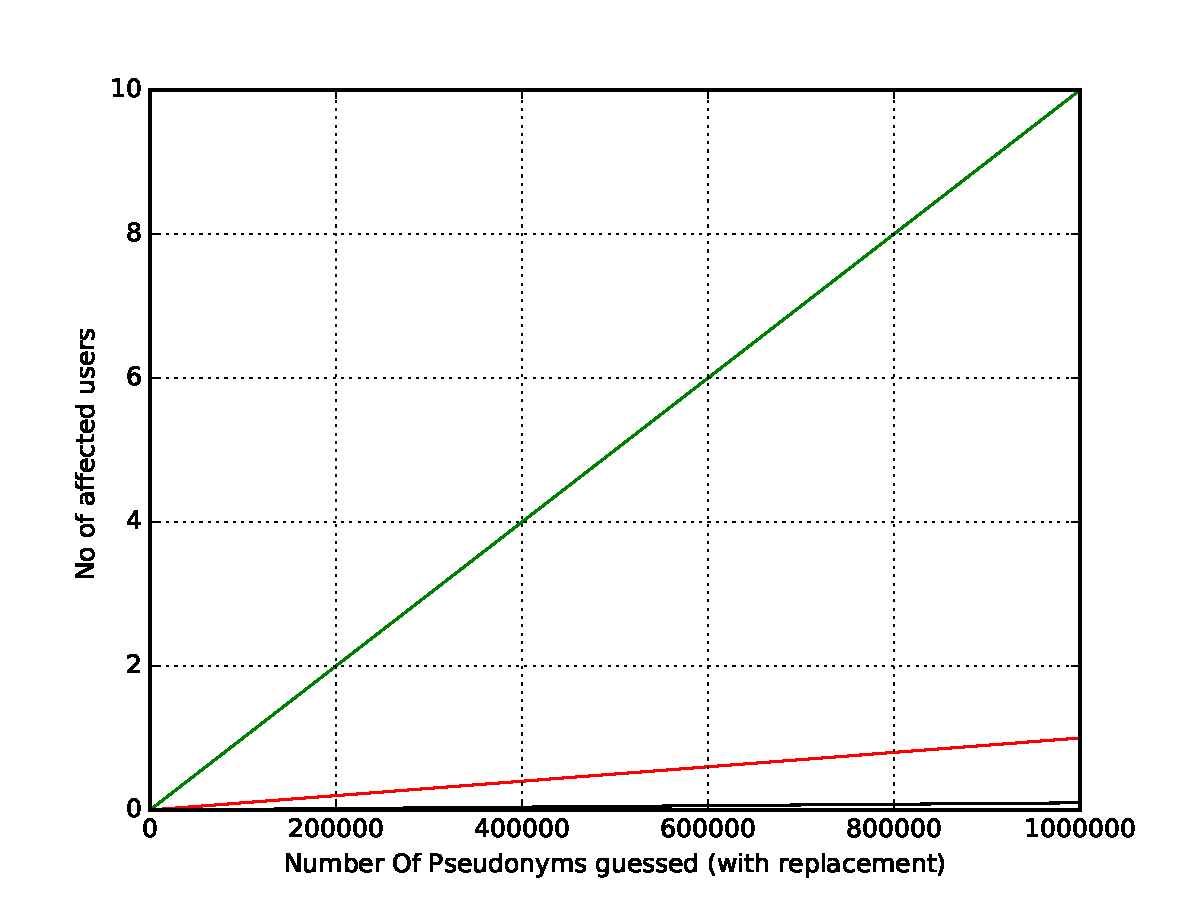
\includegraphics[width=\textwidth]{expected_success_rate_attack_by_sn_insider.pdf}
   \caption{Expected number of affected subscriber in the attack by SN. The attack is targeted to the subscribers who are visiting the SN.}
\label{fig:expected_success_rate_attack_by_sn_insider}
  \end{minipage}
  \hfill
  \begin{minipage}[b]{0.49\textwidth}
    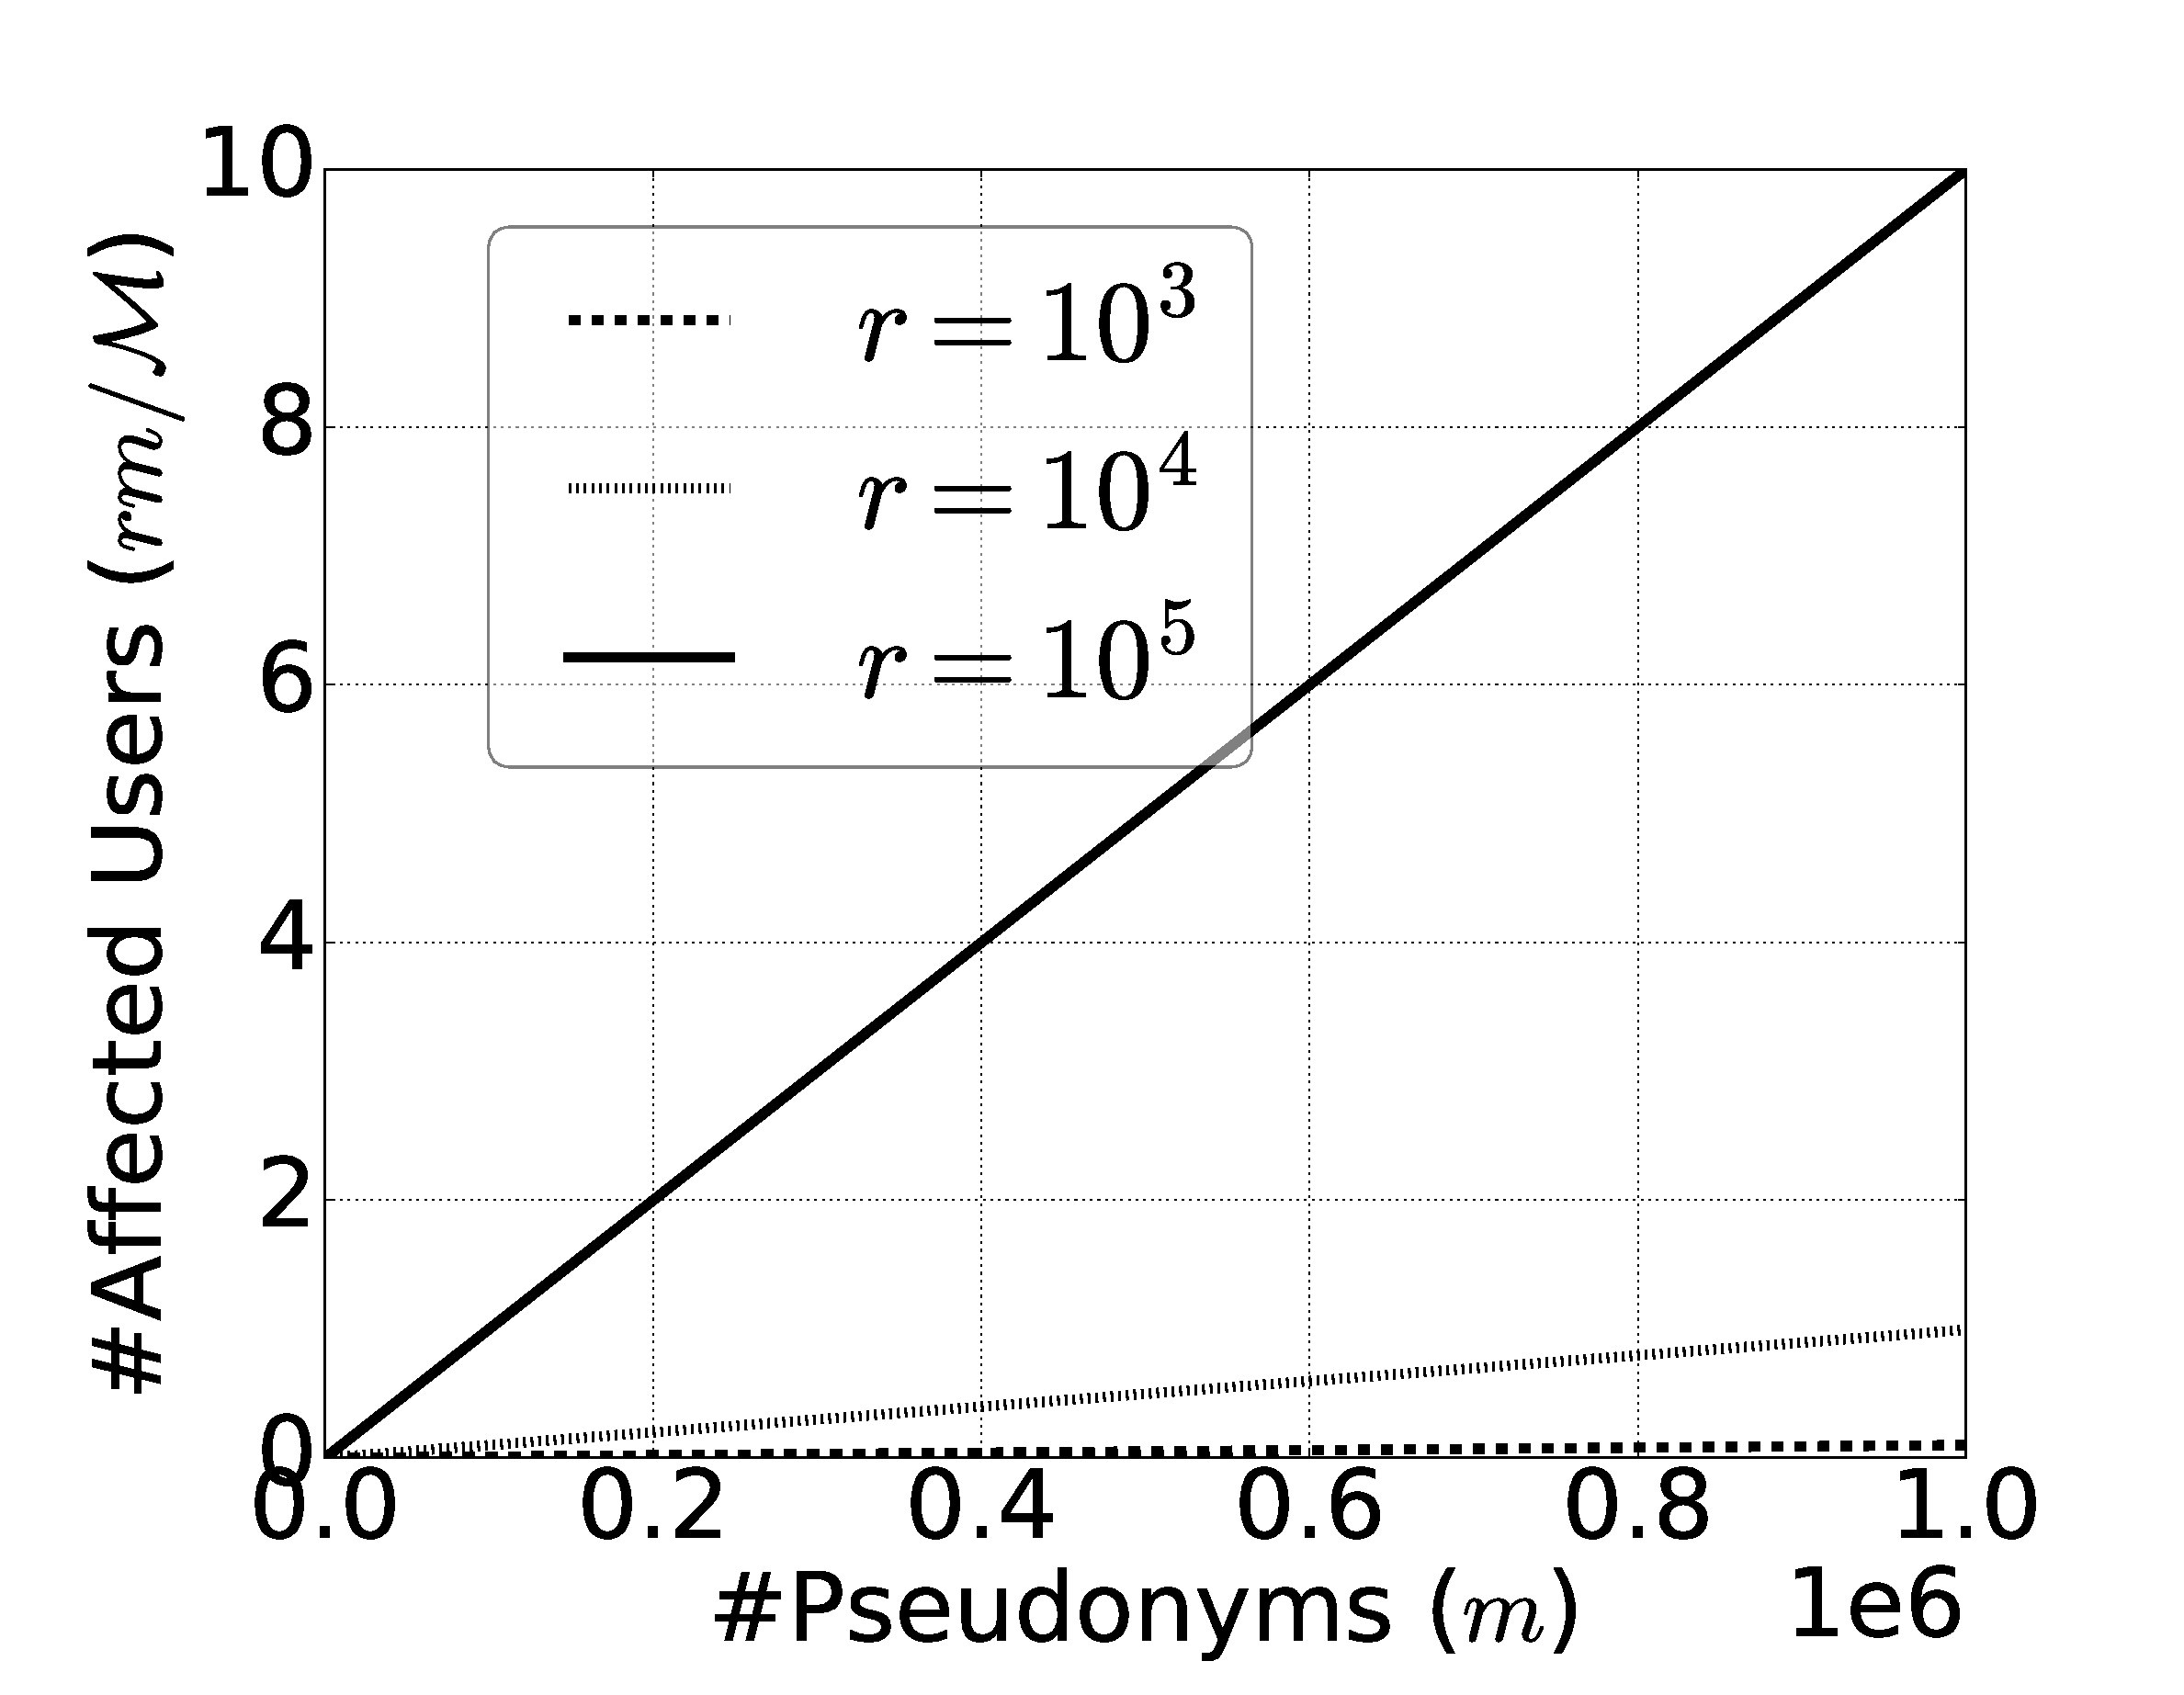
\includegraphics[width=\textwidth]{sn_attack_all.pdf}
    \caption{Expected number of affected subscriber in the attack by SN. The attack is targeted to all subscribers of the HN.}
  \label{fig:expected_success_rate_attack_all_by_sn}
  \end{minipage}
\end{figure}

\subsubsection{Target Users are not visiting the Malicious SN} The malicious SN can try to mount a DoS attack against an HN targeting the users who are not even visiting the SN. In that case, the malicious SN guesses $p''$ and send a location update for $p''$ to the SN. This bring the user to State $4$. Then the malicious SN sends an AV request to the HN using $p''$. This brings the user to State $5$. Then the SN sends another location update for $p''$. This time the user goes to State $6$. So the attack is basically a sequence of location udpate message, AV request and another location update message using the same guessed pseudonym. Let us consider that the SN starts from $0$ and choose incrementally all the possible pseudonyms across the whole space and send the three messages to the HN using the chosen pseudonym. In that way after sending $m$ triplets of messages to the HN, the expected number of affected users would be $\frac{nm}{\mathcal{M}}$. Figure \ref{fig:expected_success_rate_attack_all_by_sn} shows the expected number of affected subscribers as $m$ grows where $n$ is the total number users of an HN.

\subsection{Protection Against Replay attack by SN}
A malicious SN may store an AV that it received from the HN with an intention to use later in an AKA with a UE. If the SN could do so, then a UE can be tricked to accept an old pseudonym which is already forgotten at HN. However, an SN can not do that. Because the pseudonyms are send to the UEs encrypted. No one including the SN knows the pseudonym before it is used by a UE. Consequently the malicious SN would know a valid AV for the UE identified by pseudonym $p$ only if the AV was obtained from the HN by making an AV request using the pseudonym $p$. The next pseudonym embedded in such an AV can not be forgotten by either the UE or the HN. Hence a malicious SN can not make a replay attack to a targeted UE. However, the malicious SN can use an stored AV to run AKA with all the UE who are visiting the SN. In that case one user may get affected if the $SQN$ in the AV is still fresh. This may imply that the valid range of SQN has to be small when a UE is in roaming.

\subsection{Simplicity of the solution}

\subsection{Charging and Lawful Interception}

\subsection{Performance Overhead}

\subsection{Parameter Choice}

\subsection{Other Issues}
The encryption used in encrypting the pseudonyms will not have forward secrecy since the same key $\kappa$ is used all the time for encrypting pseudonyms. An SN may fetch multiple AVs from the HN for a single pseudonym $p$. This is not a problem because all those AVs will have the same next pseudonym embedded in them. So, once one of those AVs are used in a successful AKA, the pseudonym of the UE will change and the rest of the fetched AVs in the SN will never be used in any other AKA unless some other user in the same SN is assigned with pseudonym $p$. 

\section{Conclusion}
\label{sec:conclusion}


\subsubsection{Acknowledgement.}
\label{sec:acknowledgement}


\bibliographystyle{splncs}
\bibliography{ref}{}

\begin{thebibliography}{5}



\end{thebibliography}

\end{document}
